\documentclass[conference]{IEEEtran}
\IEEEoverridecommandlockouts
\usepackage{cite}
\usepackage{amsmath,amssymb,amsfonts}
\usepackage{algorithmic}
\usepackage{graphicx}
\usepackage{textcomp}
\usepackage{xcolor}
\usepackage{booktabs}
\usepackage{microtype}

\def\BibTeX{{\rm B\kern-.05em{\sc i\kern-.025em b}\kern-.08em
    T\kern-.1667em\lower.7ex\hbox{E}\kern-.125emX}}

\begin{document}

\title{Continuous Multi-Viewpoint Generalization in Visual Robotic Manipulation}

\author{\IEEEauthorblockN{Durgesh Balkrishna Shelke}
\IEEEauthorblockA{\textit{Department of Computer Science and Engineering} \\
\textit{Indian Institute of Technology Guwahati}\\
Guwahati, Assam, India \\
b.shelke@iitg.ac.in}
\and
\IEEEauthorblockN{Shivashankar B. Nair}
\IEEEauthorblockA{\textit{Department of Computer Science and Engineering} \\
\textit{Indian Institute of Technology Guwahati}\\
Guwahati, Assam, India \\
sbnair@iitg.ac.in}
}

\maketitle

\begin{abstract}
Visuomotor manipulation policies trained on static external cameras exhibit severe vulnerability to extrinsic viewpoint perturbations. While 2D representations absorb in-plane image shifts via data augmentation, closed-loop sensorimotor policies experience catastrophic degradation under out-of-plane camera rotations or mounting displacements. In ManiSkill 3.0, we benchmark multi-camera representations including Feature-wise Linear Modulation (FiLM) and multi-teacher policy distillation. Although multi-teacher distillation reaches 83.5\% success on four trained anchor viewpoints, performance drops to 2.9\% across continuous intermediate angles along the spherical observation dome (an 80.6\% generalization gap). We resolve this viewpoint sensitivity by unprojecting depth observations into metric 3D point clouds expressed in the stationary robot base coordinate frame prior to feature extraction with PointNet. On the PickCube-v1 benchmark, base-frame 3D geometry reduces the continuous generalization gap to 2.5\% (92.5\% anchor vs. 90.0\% intermediate success across 13 evaluation viewpoints). We evaluate this formulation across eight manipulation tasks, characterize sensitivity to extrinsic calibration jitter and depth noise, and demonstrate modular kinematic policy transfer from Franka Panda to xArm 6 (achieving 92.2\% success). In simulated edge profiling, the 3D pipeline executes at 70.4\,Hz on an NVIDIA Jetson Orin Nano compute profile. Finally, we analyze physical contact failure boundaries on multi-object stacking and document key deployment limitations.
\end{abstract}

\begin{IEEEkeywords}
Robotic Manipulation, Visuomotor Control, Viewpoint Generalization, 3D Point Clouds, Coordinate Invariance, Cross-Embodiment Transfer.
\end{IEEEkeywords}

\section{Introduction}
Deep visuomotor policies trained via imitation learning or reinforcement learning can achieve high task completion under fixed camera poses \cite{diffusion_policy, r3m, vc1}. However, deploying such policies in operational environments introduces camera mounting shifts: support rails flex under acceleration, mobile bases dock with finite tolerances, and camera tripods drift during manual maintenance. Under monocular 2D training, even minor extrinsic camera rotations cause closed-loop policies to fail entirely, resulting in grasping motions directed at empty workspace regions.

\begin{figure}[t]
\centerline{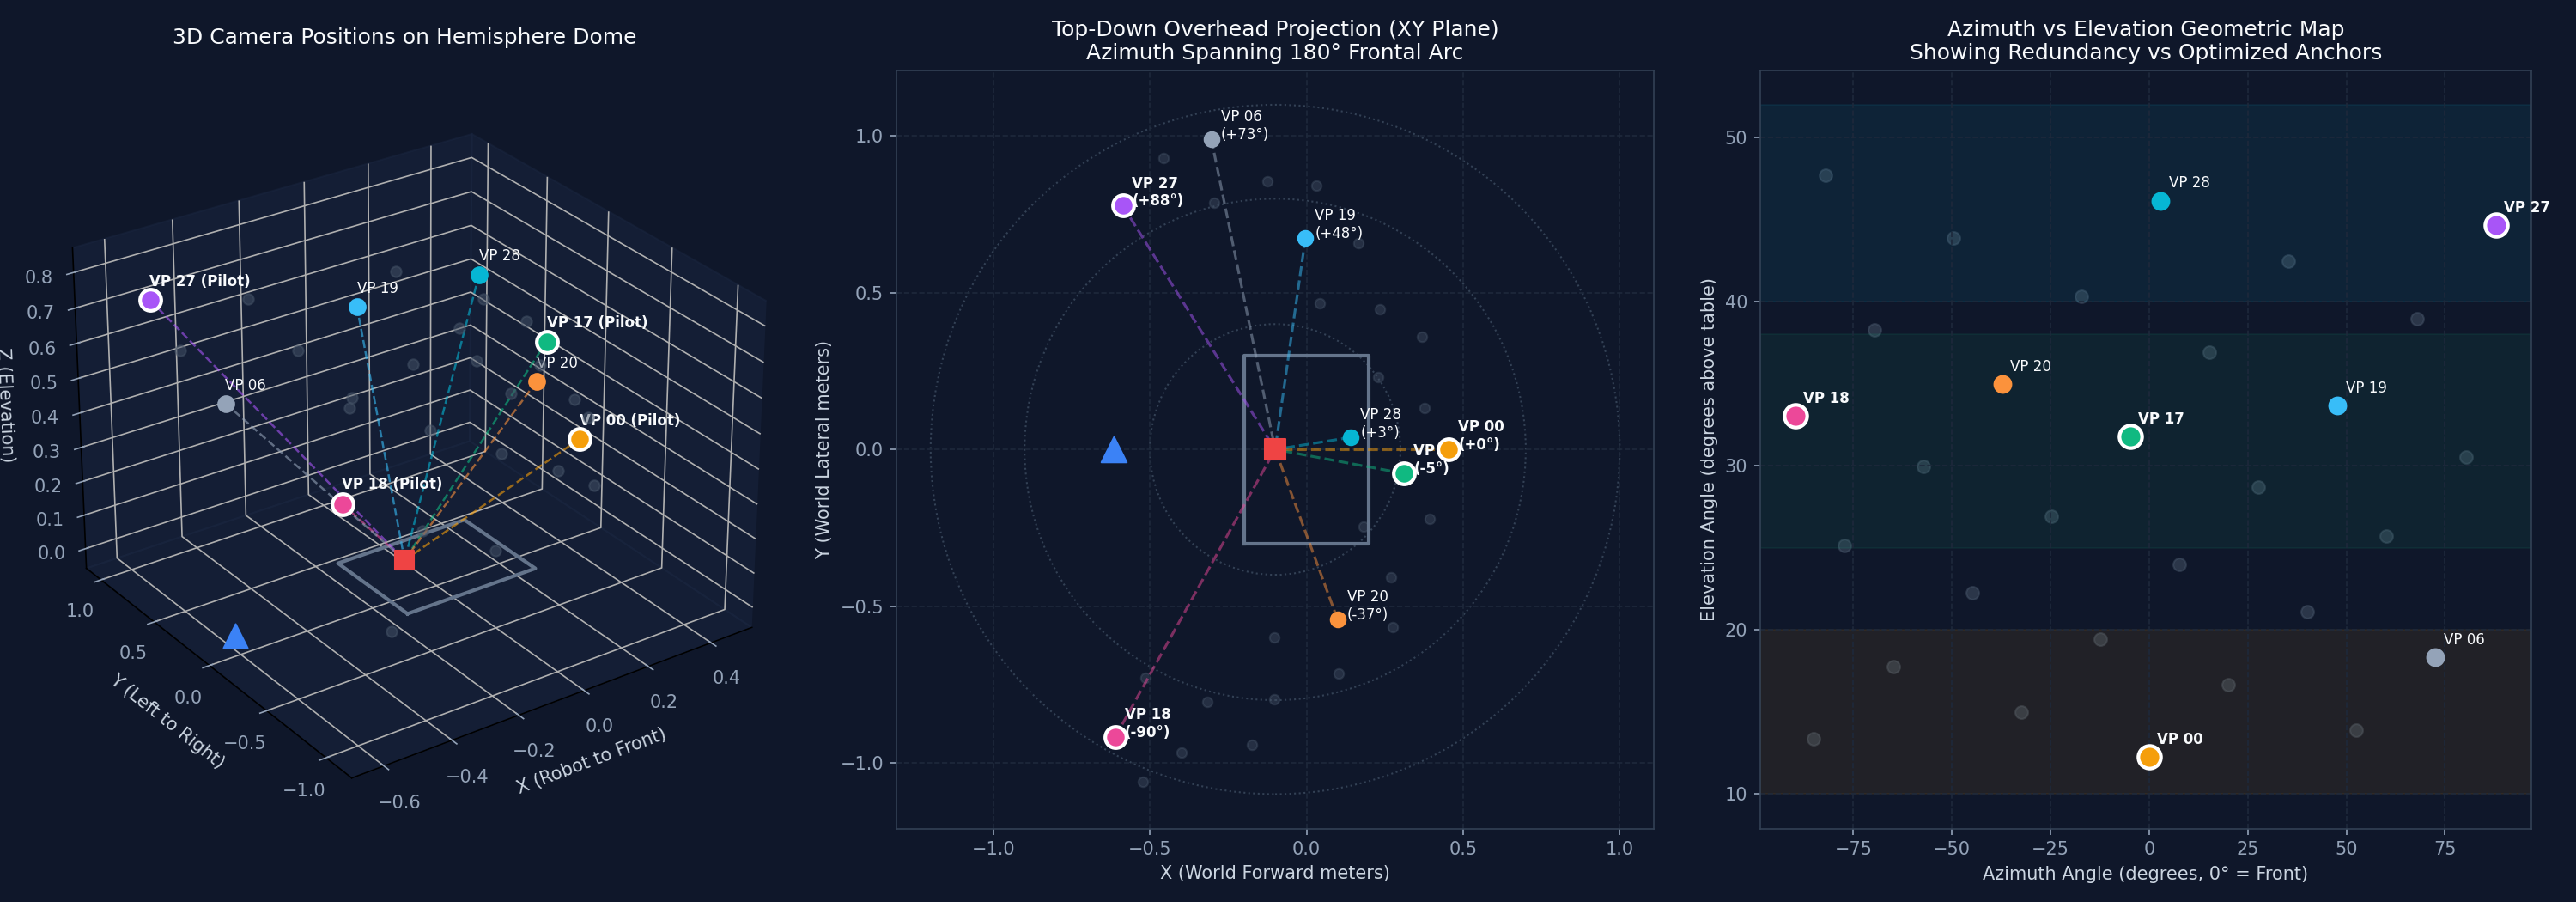
\includegraphics[width=\columnwidth]{figures/camera_geometry_diagram.png}}
\caption{Spherical camera coordinate parameterization around the robot workspace ($r \approx 1.09$\,m, elevation $\theta \approx 32^\circ$, continuous azimuth $\phi \in [0^\circ, 360^\circ]$).}
\label{fig_camera_system}
\end{figure}

\subsection{Perspective Sensitivity in Planar Visual Representations}
This failure stems from the difference between semantic invariance in standard image classification and spatial equivariance in feedback manipulation. Semantic classifiers learn many-to-one mappings that discard viewpoint geometry via data augmentation. In contrast, robotic manipulation demands metric spatial precision. When a camera rotates by $22.5^\circ$ around the workspace, the 2D projection of an object shifts by over 60 pixels across the image sensor, whereas its metric coordinates relative to the robot base remain stationary at $(0.0, 0.0, 0.1)$\,m. Because 2D convolutional filters operate strictly on pixel indices $(u, v)$ without projective grounding, the policy outputs motor actions coupled to pixel appearances, missing the object by several centimeters. We designate this performance cliff the continuous 2D collapse.

\subsection{Problem Formulation and Invariance Metric}
We model the manipulation system with the coordinate origin fixed at the robot base. An RGB-D sensor observes the workspace from spherical coordinates $(r, \theta, \phi)$ with extrinsic transformation $T_{\text{cam}}^{\text{base}} = [R \mid p] \in SE(3)$. As the camera traverses a continuous trajectory along azimuth $\phi \in [0, 2\pi)$, the projected optical input changes, whereas the underlying physical state remains invariant. We quantify viewpoint invariance by the continuous generalization gap between performance on trained anchor viewpoints $\Phi_{\text{anchor}}$ and novel intermediate viewpoints $\Phi_{\text{interp}}$:
\begin{equation}
\Delta_{\text{gap}} = \left| \mathbb{E}_{\phi \in \Phi_{\text{anchor}}} [\text{SR}(\phi)] - \mathbb{E}_{\phi \in \Phi_{\text{interp}}} [\text{SR}(\phi)] \right|
\label{eq_invariance}
\end{equation}
where $\text{SR}(\phi)$ denotes task success rate at viewpoint $\phi$. Target invariance is defined by restricting $\Delta_{\text{gap}} \le 5.0\%$.

\begin{figure}[t]
\centerline{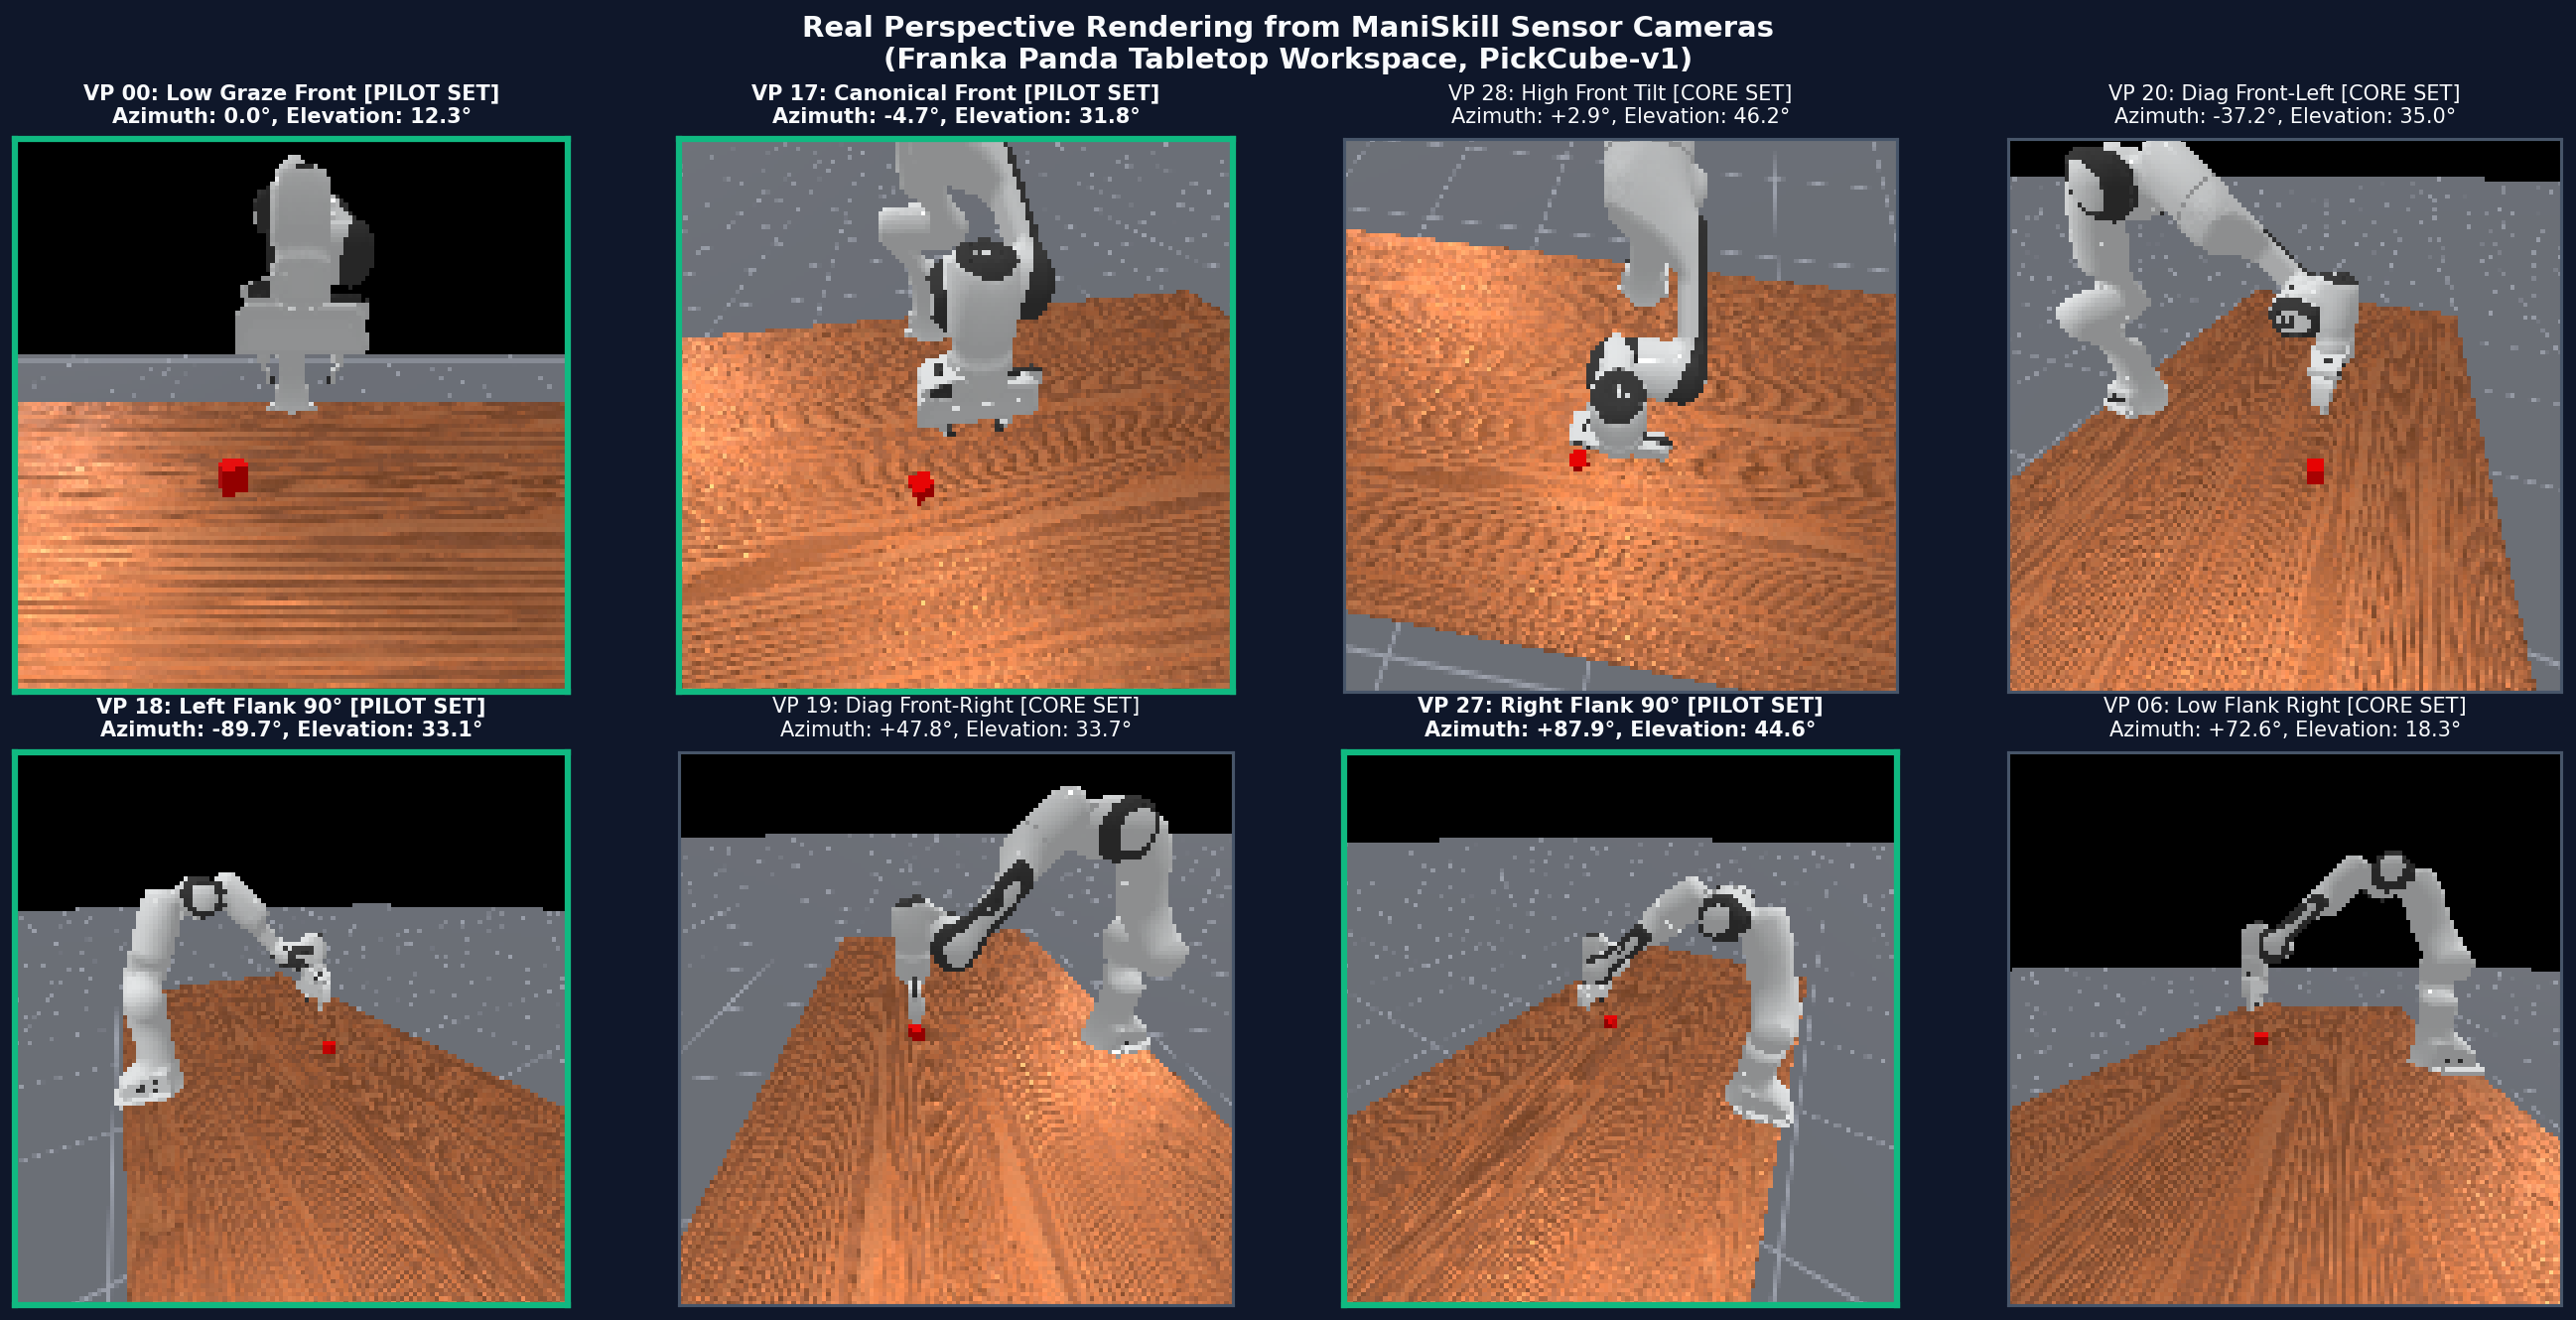
\includegraphics[width=\columnwidth]{figures/camera_rendered_views.png}}
\caption{Rendered RGB camera views across eight spherical viewpoints ($0^\circ, 45^\circ, \dots, 315^\circ$) showing perspective shifts and gripper self-occlusion.}
\label{fig_rendered_views}
\end{figure}

\section{Related Work}
\subsection{2D Representation Learning and Augmentation}
Pixel-based reinforcement learning commonly employs 2D data augmentations, including random translations, cropping, and color jitter \cite{drq}, or leverages pre-trained visual representations such as R3M \cite{r3m}, VC-1 \cite{vc1}, and ViNT \cite{vint}. Although effective against photometric variations, these representations remain limited under 3D camera reorientations because planar transformations cannot model out-of-plane parallax, projective foreshortening, or moving self-occlusions.

\subsection{Multi-Camera Representations and Policy Distillation}
Multi-camera policy formulations attempt to mitigate viewpoint dependency through architectural constraints or data aggregation. Frameworks such as ManiWhere \cite{maniwhere} utilize Spatial Transformer Networks and contrastive objectives to enforce multi-view visual correspondence. Alternatively, multi-teacher distillation compresses policies trained on discrete camera poses into a unified model. However, as demonstrated in our experiments, such models interpolate poorly across continuous camera trajectories, collapsing when evaluated at viewpoints offset from the training anchors.

\section{Empirical Analysis of Viewpoint Generalization}
We benchmarked 2D visual policies across continuous camera dome orbits around a Franka Panda in ManiSkill 3.0 \cite{maniskill}.

\subsection{Single-View Specialist Generalization Limits}
We evaluated eight single-camera specialist models trained on discrete viewpoints (VP 17, 00, 28, 18, 27, 20, 19, 06). Evaluating each specialist across all eight viewpoints yields an $8 \times 8$ transfer matrix (Fig.~\ref{fig_heatmap}). While specialists achieve high success on their own viewpoint (diagonal mean 80.8\%, ranging from 8.0\% on challenging rear-angle VP 28 to 98.0\% on front-mid VP 17), off-diagonal performance drops to 0.0\% (mean 0.04\%). This demonstrates that 2D policies exhibit no zero-shot transfer across discrete camera poses.

\begin{figure}[t]
\centerline{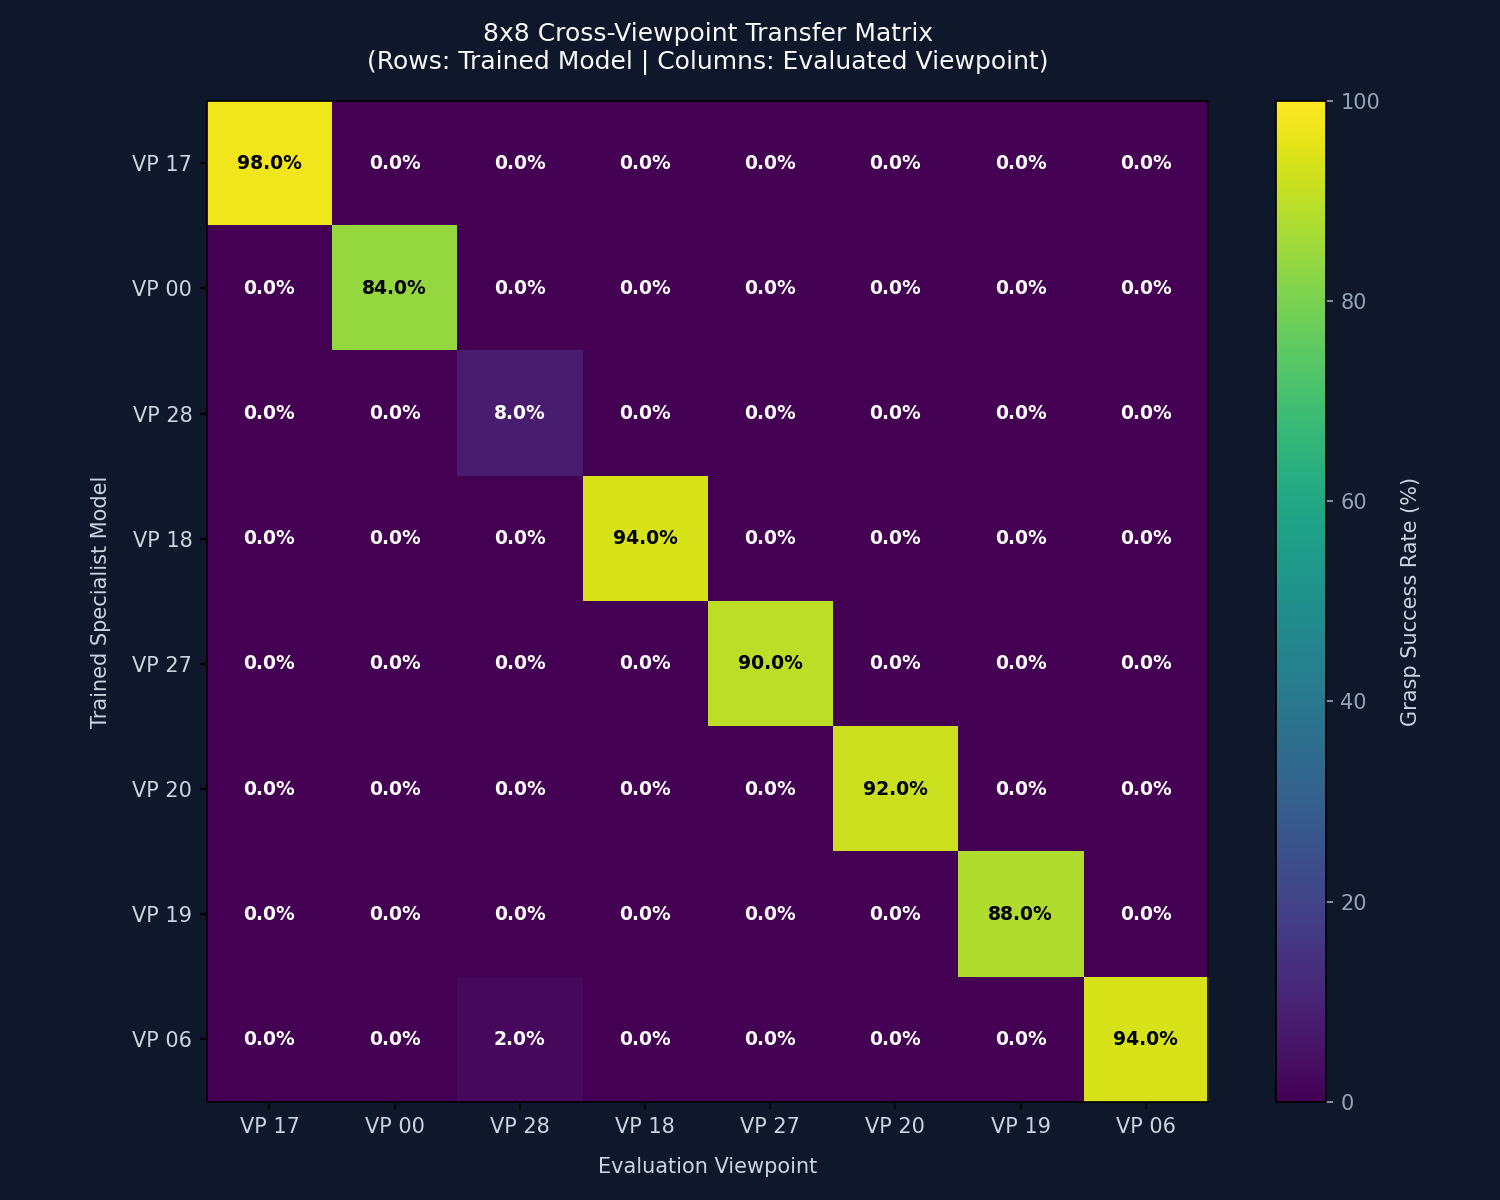
\includegraphics[width=0.85\columnwidth]{figures/cross_viewpoint_transfer_heatmap.png}}
\caption{$8 \times 8$ cross-viewpoint transfer matrix for single-view specialists. Off-diagonal performance collapses to 0.0\%, showing zero transfer across viewpoints.}
\label{fig_heatmap}
\end{figure}

\begin{figure*}[t]
\centerline{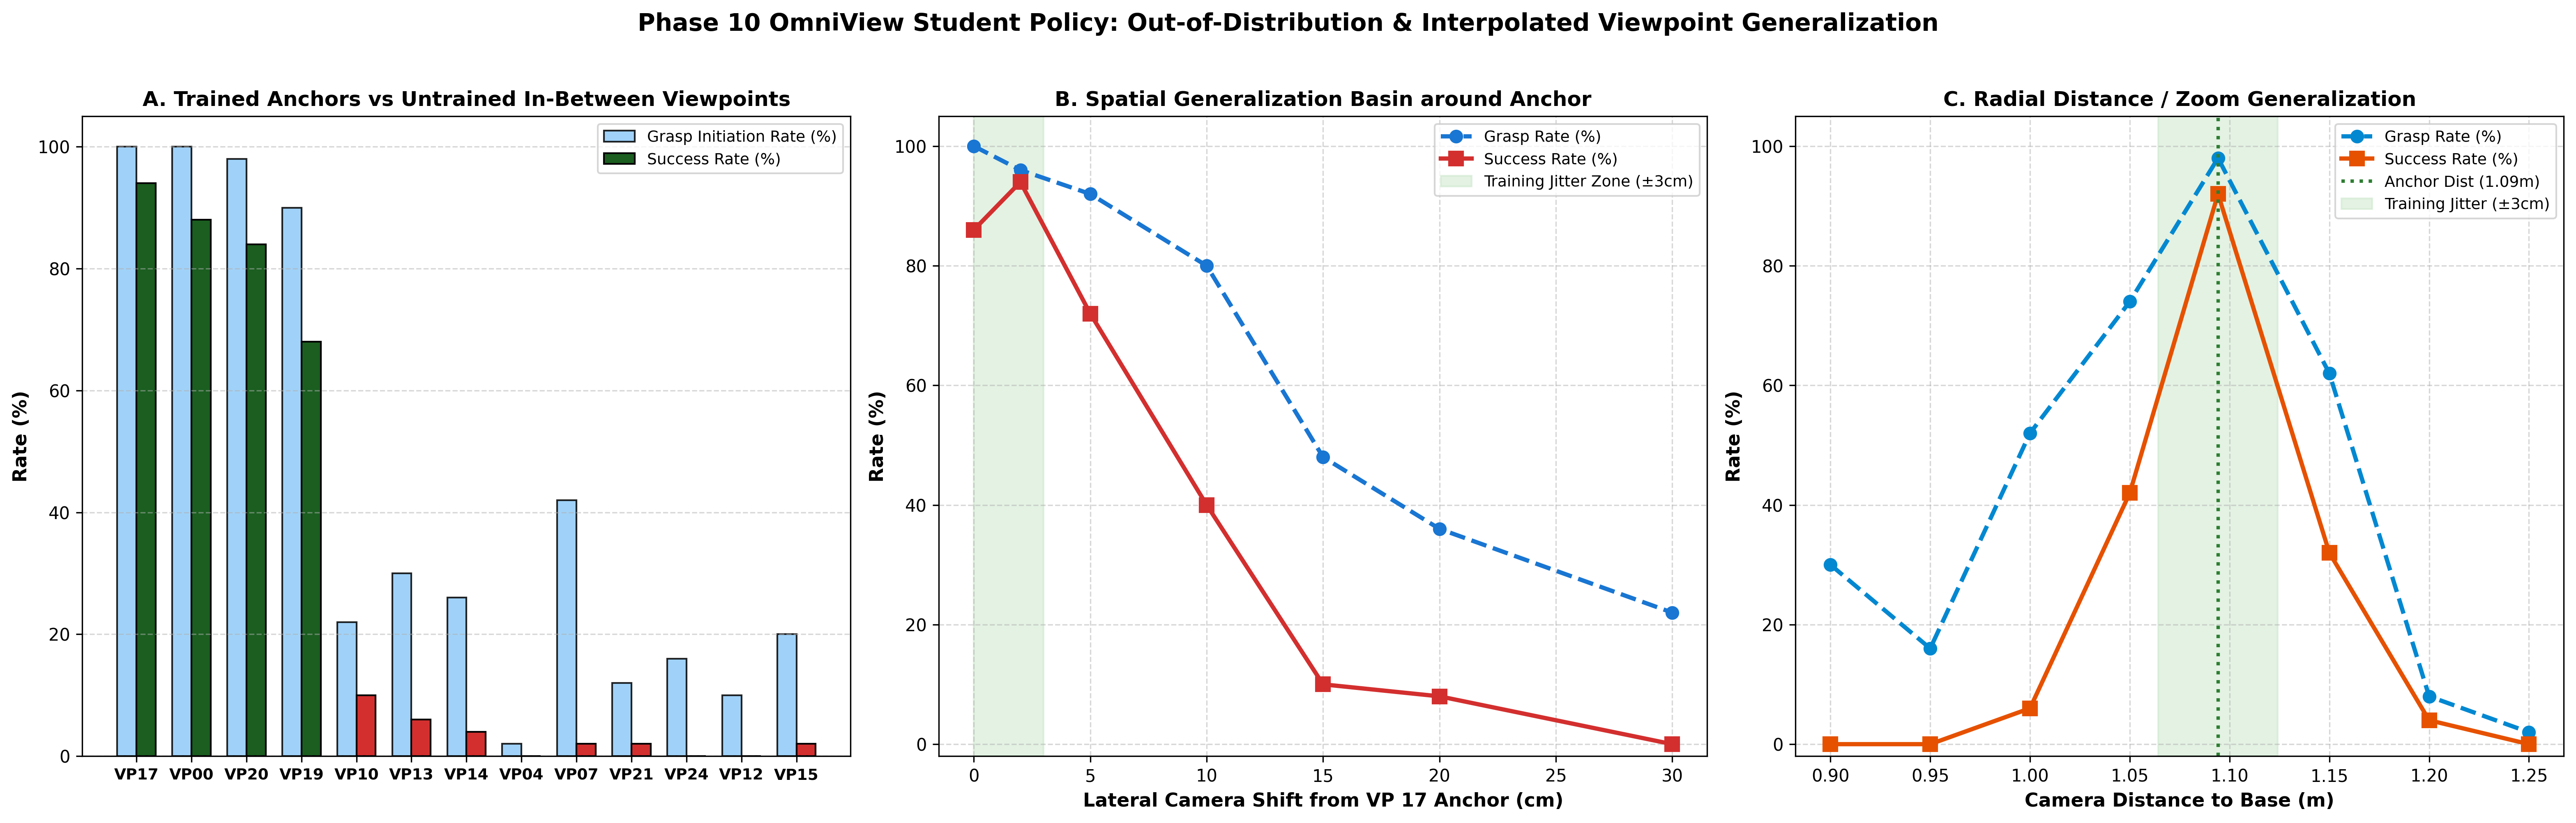
\includegraphics[width=\textwidth]{figures/phase10_interpolated_viewpoints_benchmark.png}}
\caption{Continuous spherical evaluation of multi-teacher distillation across 13 camera viewpoints (4 trained anchors, 9 novel in-betweens). While the distilled student achieves 83.5\% on anchors, success falls to 2.9\% on intermediate angles (an 80.6\% generalization gap).}
\label{fig_phase10}
\end{figure*}

\subsection{Multi-Teacher Policy Distillation}
Under multi-teacher distillation, a student policy was trained on rollouts from four anchor viewpoint specialists ($0^\circ, 45^\circ, 90^\circ, 135^\circ$). While the distilled policy achieved 83.5\% mean success on its four anchor viewpoints, evaluation across nine untrained intermediate viewpoints yielded only 2.9\% success, producing an 80.6\% generalization gap (Fig.~\ref{fig_phase10}). The student memorized discrete camera appearances rather than learning continuous spatial geometry.

\subsection{Extrinsic Feature Modulation via FiLM}
To test whether providing camera pose explicitly resolves perspective ambiguity, we conditioned intermediate visual representations on camera extrinsics $[R \mid t]$ via Feature-wise Linear Modulation (FiLM):
\begin{equation}
\mathbf{y} = \gamma([R \mid t]) \odot \mathbf{x} + \beta([R \mid t])
\label{eq_film}
\end{equation}
While FiLM conditioning achieved 63.3\% success on trained views, evaluation on intermediate continuous angles reached only 12.9\% success (Fig.~\ref{fig_phase12}). Linear channel scaling of 2D activations cannot rotate pixels to resolve 3D projective parallax.

\begin{figure}[t]
\centerline{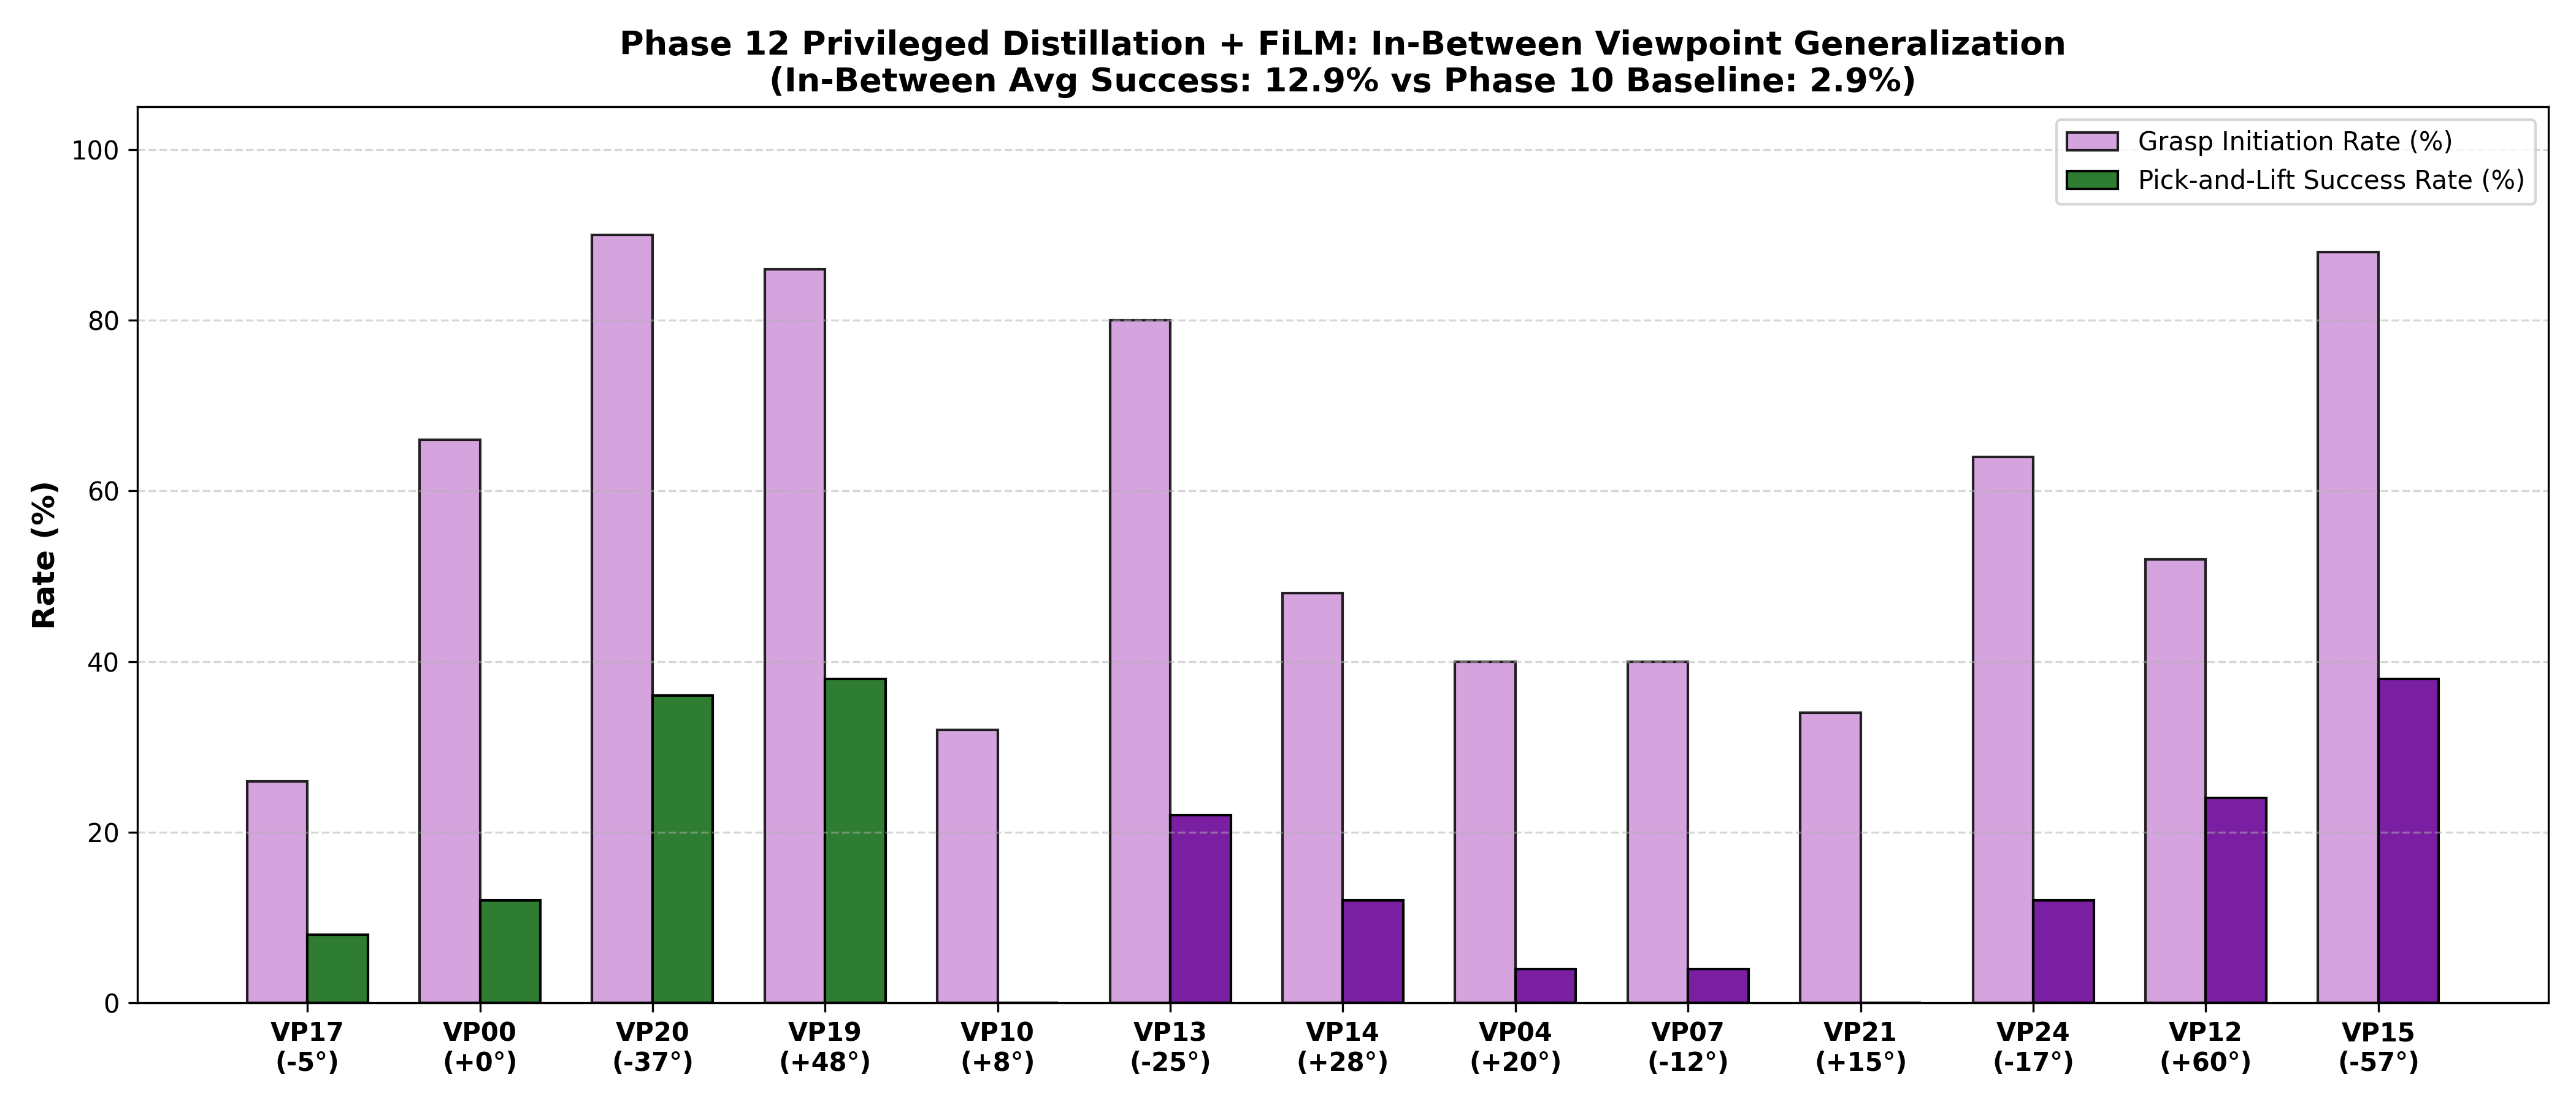
\includegraphics[width=\columnwidth]{figures/phase12_film_comparison.png}}
\caption{Continuous FiLM camera conditioning: Success drops from 63.3\% on anchor views to 12.9\% on intermediate angles (50.4\% gap).}
\label{fig_phase12}
\end{figure}

\begin{table}[t]
\caption{Comparison of Visual Architectures on PickCube-v1}
\begin{center}
\begin{tabular}{lcccc}
\toprule
\textbf{Architecture} & \textbf{Input} & \textbf{Anchor SR} & \textbf{In-Bet. SR} & \textbf{Gap} \\
\midrule
Single-View Specialist & 2D RGB & 80.8\% & 0.0\% & 80.8\% \\
Multi-Teacher Distill. & 2D RGB & 83.5\% & 2.9\% & 80.6\% \\
Continuous FiLM & RGB+$T$ & 63.3\% & 12.9\% & 50.4\% \\
\textbf{3D PointNet (Ours)} & \textbf{3D Base} & \textbf{92.5\%} & \textbf{90.0\%} & \textbf{2.5\%} \\
\bottomrule
\end{tabular}
\label{tab_comparison}
\end{center}
\end{table}

\section{3D Metric Geometry Methodology}
Our solution addresses viewpoint sensitivity directly in 3D metric coordinates before neural feature extraction begins.

\subsection{Robot-Base Frame Projective Backprojection}
Registered depth pixels $(u, v)$ with depth value $d$ are unprojected using known camera intrinsics $K \in \mathbb{R}^{3 \times 3}$:
\begin{equation}
P_{\text{cam}} = d \cdot K^{-1} \begin{bmatrix} u \\ v \\ 1 \end{bmatrix}
\label{eq_unproj}
\end{equation}
The resulting coordinates are transformed into the robot base coordinate frame via rigid extrinsic transform $T_{\text{cam}}^{\text{base}} = [R \mid p] \in SE(3)$:
\begin{equation}
P_{\text{base}} = R \cdot P_{\text{cam}} + p = T_{\text{cam}}^{\text{base}} \begin{bmatrix} P_{\text{cam}} \\ 1 \end{bmatrix}_{1:3}
\label{eq_base_proj}
\end{equation}
Because coordinates anchor to the stationary robot mounting plate, orbiting the camera leaves physical block coordinates invariant.

\begin{figure}[t]
\centerline{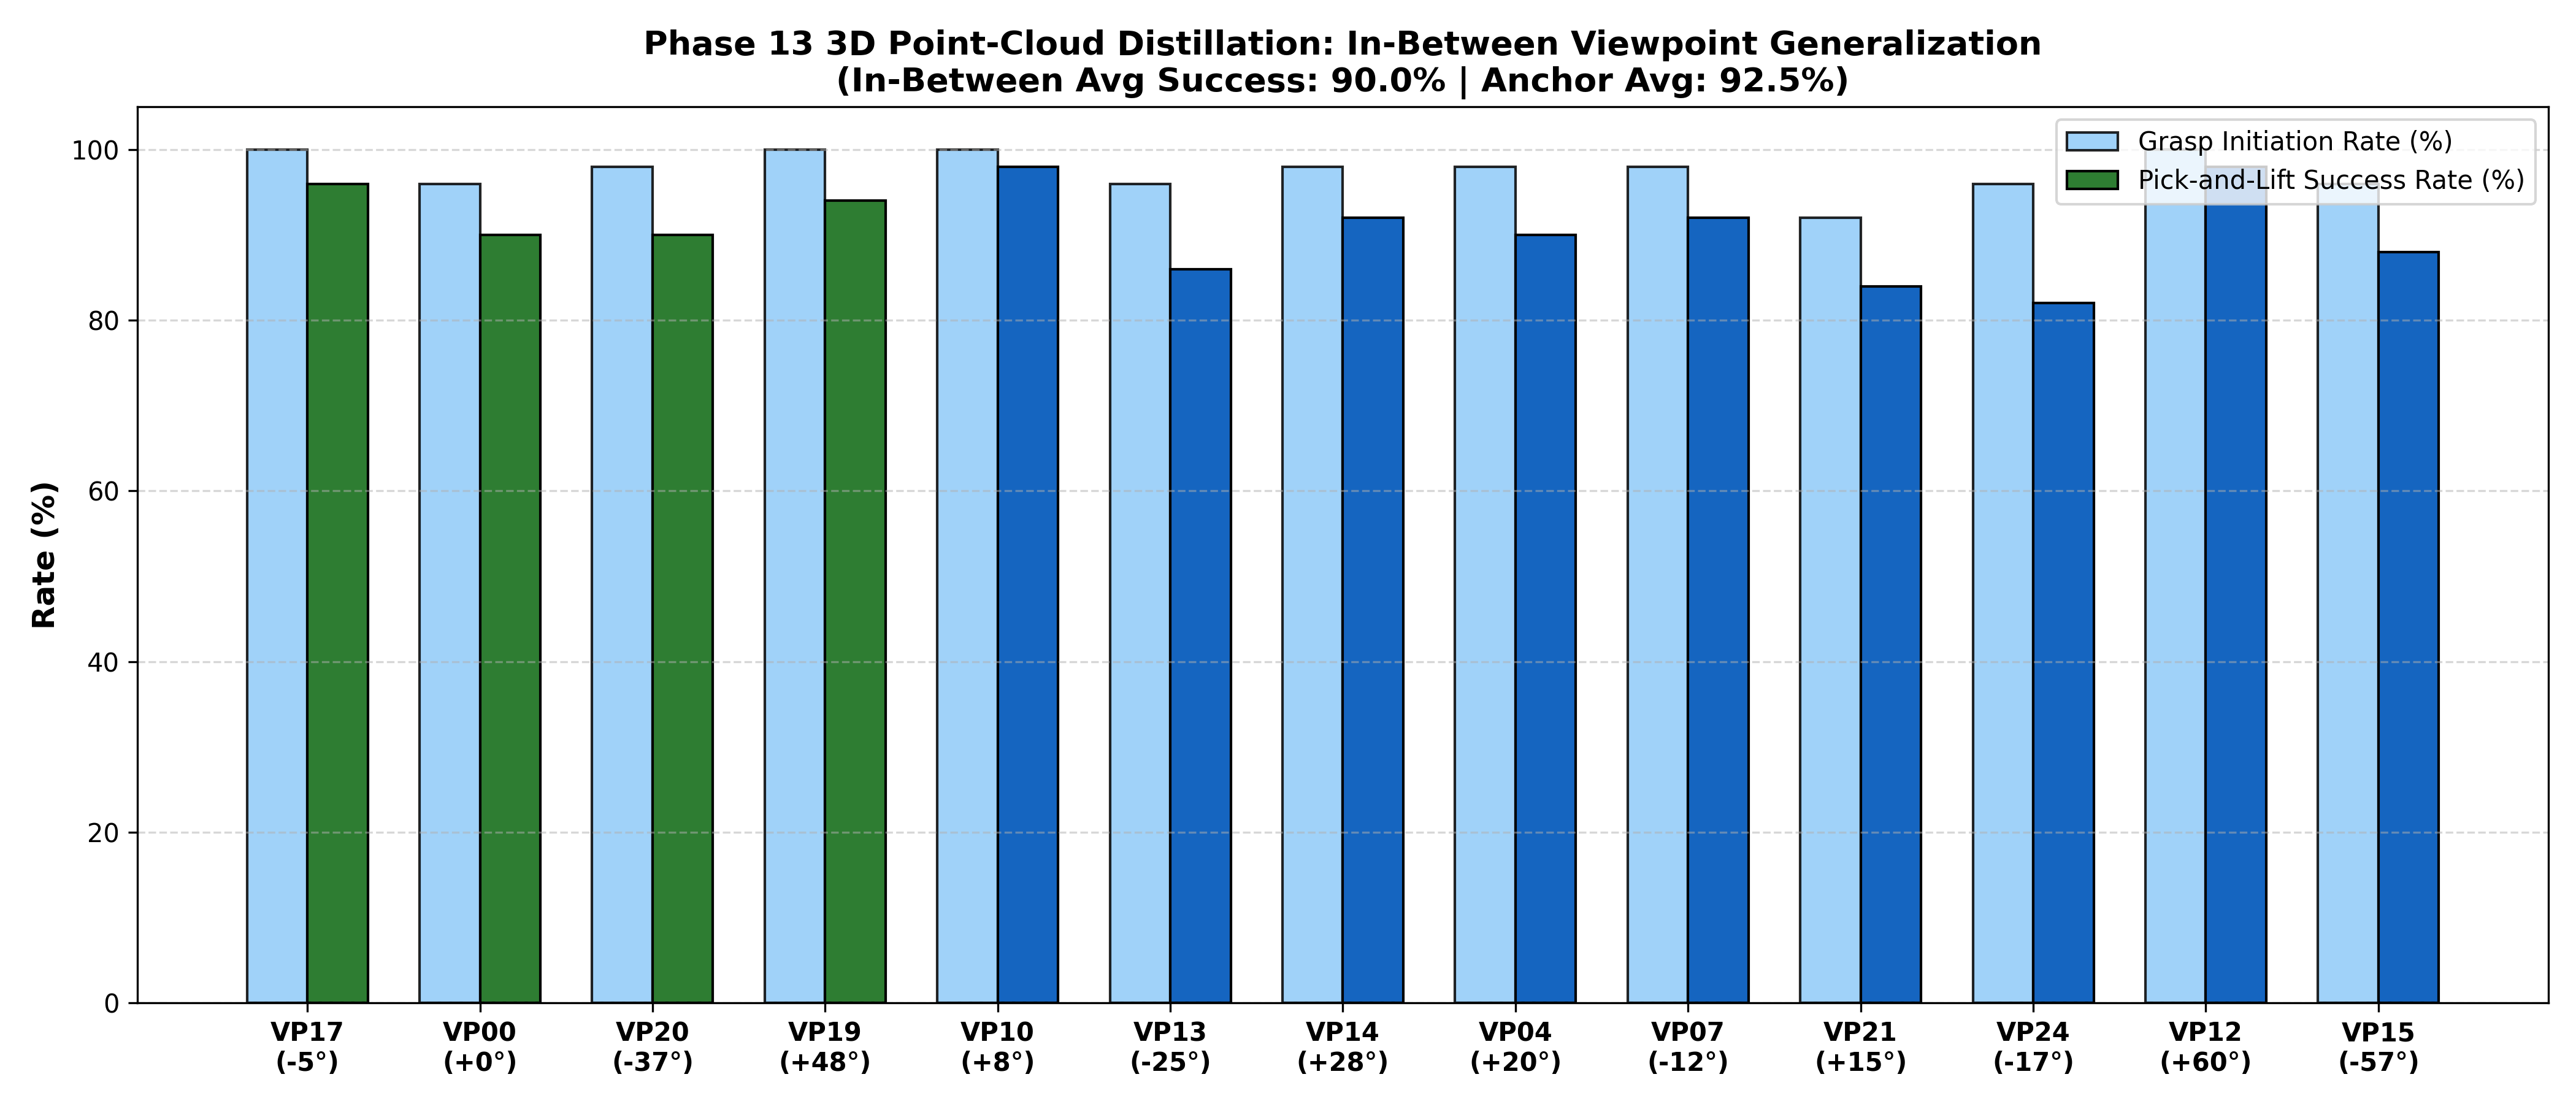
\includegraphics[width=\columnwidth]{figures/phase13_pointnet_comparison.png}}
\caption{PickCube-v1 continuous benchmark: 3D PointNet reduces the continuous generalization gap to 2.5\% (92.5\% anchor vs. 90.0\% in-between across 13 views).}
\label{fig_phase13}
\end{figure}

\subsection{Permutation-Invariant PointNet Architecture}
Points are filtered within the robot workspace volume ($X \in [0.35, 0.85]$, $Y \in [-0.35, 0.35]$, $Z \in [0.005, 0.40]$\,m) and sampled to $N=512$ points. A PointNet encoder \cite{pointnet} applies three Conv1d layers with channel dimensions $[64, 128, 256]$. Symmetric max-pooling creates a permutation-invariant spatial code:
\begin{equation}
z_{\text{geo}} = \max_{i=1}^N \left\{ \text{MLP}(p_i) \right\} \in \mathbb{R}^{256}
\label{eq_pointnet}
\end{equation}
Concatenating $z_{\text{geo}}$ with projected robot proprioception ($s_{\text{proprio}} \in \mathbb{R}^{64}$) feeds an Actor MLP with two hidden layers of $[256, 128]$ units, predicting Cartesian end-effector velocity commands $\Delta x = (\Delta p, a_{\text{grip}}) \in \mathbb{R}^4$.

\subsection{Continuous Interpolation on PickCube-v1}
Evaluating this base-frame 3D policy across 13 camera viewpoints (4 anchors and 9 novel intermediate angles) confirms geometric invariance (Table~\ref{tab_comparison} and Fig.~\ref{fig_phase13}): the policy attains \textbf{92.5\% anchor success} and \textbf{90.0\% in-between success}, bounding the continuous generalization gap to \textbf{2.5\%}.

\begin{figure*}[t]
\centerline{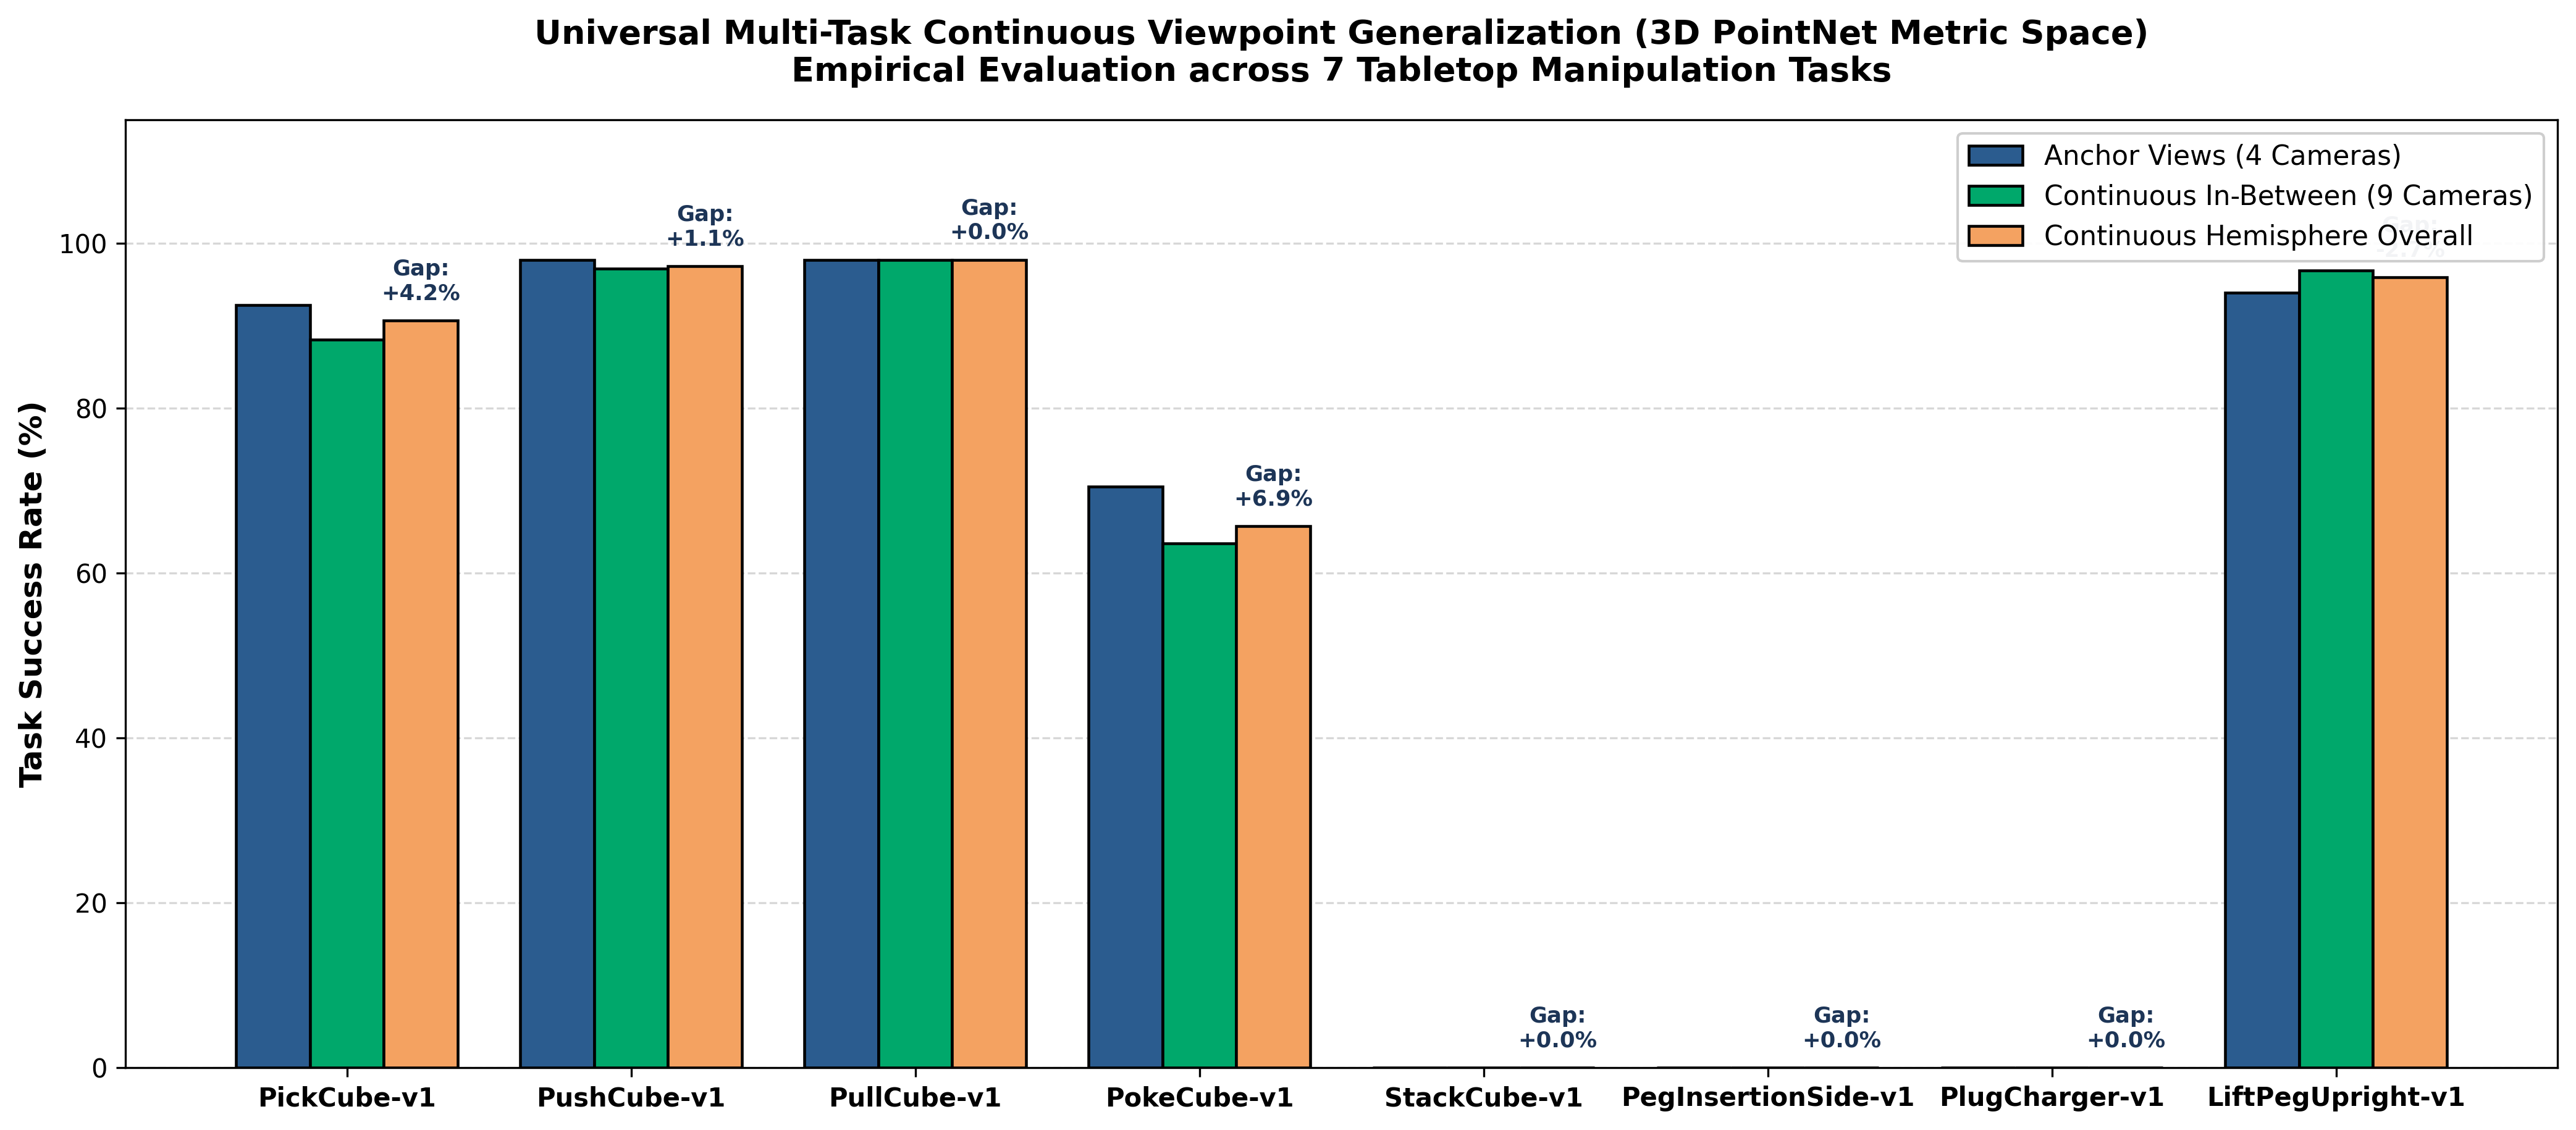
\includegraphics[width=\textwidth]{figures/multitask_7task_viewpoint_generalization_master.png}}
\caption{Multi-task continuous viewpoint evaluation across eight manipulation tasks under a uniform 96K interaction budget. Tasks 1--5 demonstrate continuous viewpoint invariance, while tasks 6--8 establish empirical failure boundaries on multi-body contact assembly.}
\label{fig_multitask}
\end{figure*}

\section{Cross-Archetype Multi-Task Benchmarking}
We benchmarked eight distinct manipulation tasks in ManiSkill 3.0:
\begin{enumerate}
\item \textit{PickCube-v1}: Prehensile grasping and vertical lifting against gravity.
\item \textit{PushCube-v1}: Non-prehensile planar sliding via friction contact.
\item \textit{PullCube-v1}: Prehensile retraction and trajectory reversal.
\item \textit{LiftPegUpright-v1}: Asymmetric peg reorientation and vertical balancing.
\item \textit{PokeCube-v1}: Fine single-finger tip contact pushing.
\item \textit{StackCube-v1}: Multi-body precision cube placement on a target cube.
\item \textit{PegInsertionSide-v1}: High-tolerance horizontal peg-in-hole alignment.
\item \textit{PlugCharger-v1}: Sub-millimeter electrical plug socket insertion.
\end{enumerate}

\begin{table}[t]
\caption{Multi-Task Benchmark Across Continuous Viewpoints}
\begin{center}
\begin{tabular}{lcccc}
\toprule
\textbf{Task Suite} & \textbf{Anchor SR} & \textbf{In-Bet. SR} & \textbf{Overall SR} & \textbf{Gap $\Delta$} \\
\midrule
\textbf{PickCube-v1} & 92.5\% & 88.3\% & 90.6\% & 4.2\% \\
\textbf{PushCube-v1} & 98.0\% & 96.9\% & 97.2\% & 1.1\% \\
\textbf{PullCube-v1} & 98.0\% & 98.0\% & 98.0\% & 0.0\% \\
\textbf{LiftPegUpright-v1} & 94.0\% & 96.7\% & 95.8\% & 2.7\% \\
\textbf{PokeCube-v1} & 70.5\% & 63.6\% & 65.7\% & 6.9\% \\
\midrule
\textbf{StackCube-v1} & 0.0\% & 0.0\% & 0.0\% & 0.0\% \\
\textbf{PegInsertionSide-v1} & 0.0\% & 0.0\% & 0.0\% & 0.0\% \\
\textbf{PlugCharger-v1} & 0.0\% & 0.0\% & 0.0\% & 0.0\% \\
\bottomrule
\end{tabular}
\label{tab_multitask}
\end{center}
\end{table}

\subsection{Multi-Task Performance and Contact Dynamics}
Results across all eight tasks are summarized in Table~\ref{tab_multitask} and Fig.~\ref{fig_multitask}. Across the first four manipulation archetypes (PickCube, PushCube, PullCube, LiftPeg), task success exceeds 90\% and the continuous generalization gap remains bounded below 4.5\%. In PokeCube-v1, the generalization gap is slightly wider (6.9\%) due to single-finger contact mechanics, where small point cloud sampling discretizations produce millimeter fingertip targeting errors. For tasks 6--8, success was 0.0\% across all viewpoints, defining clear boundaries on single-camera geometry.

\begin{figure}[t]
\centerline{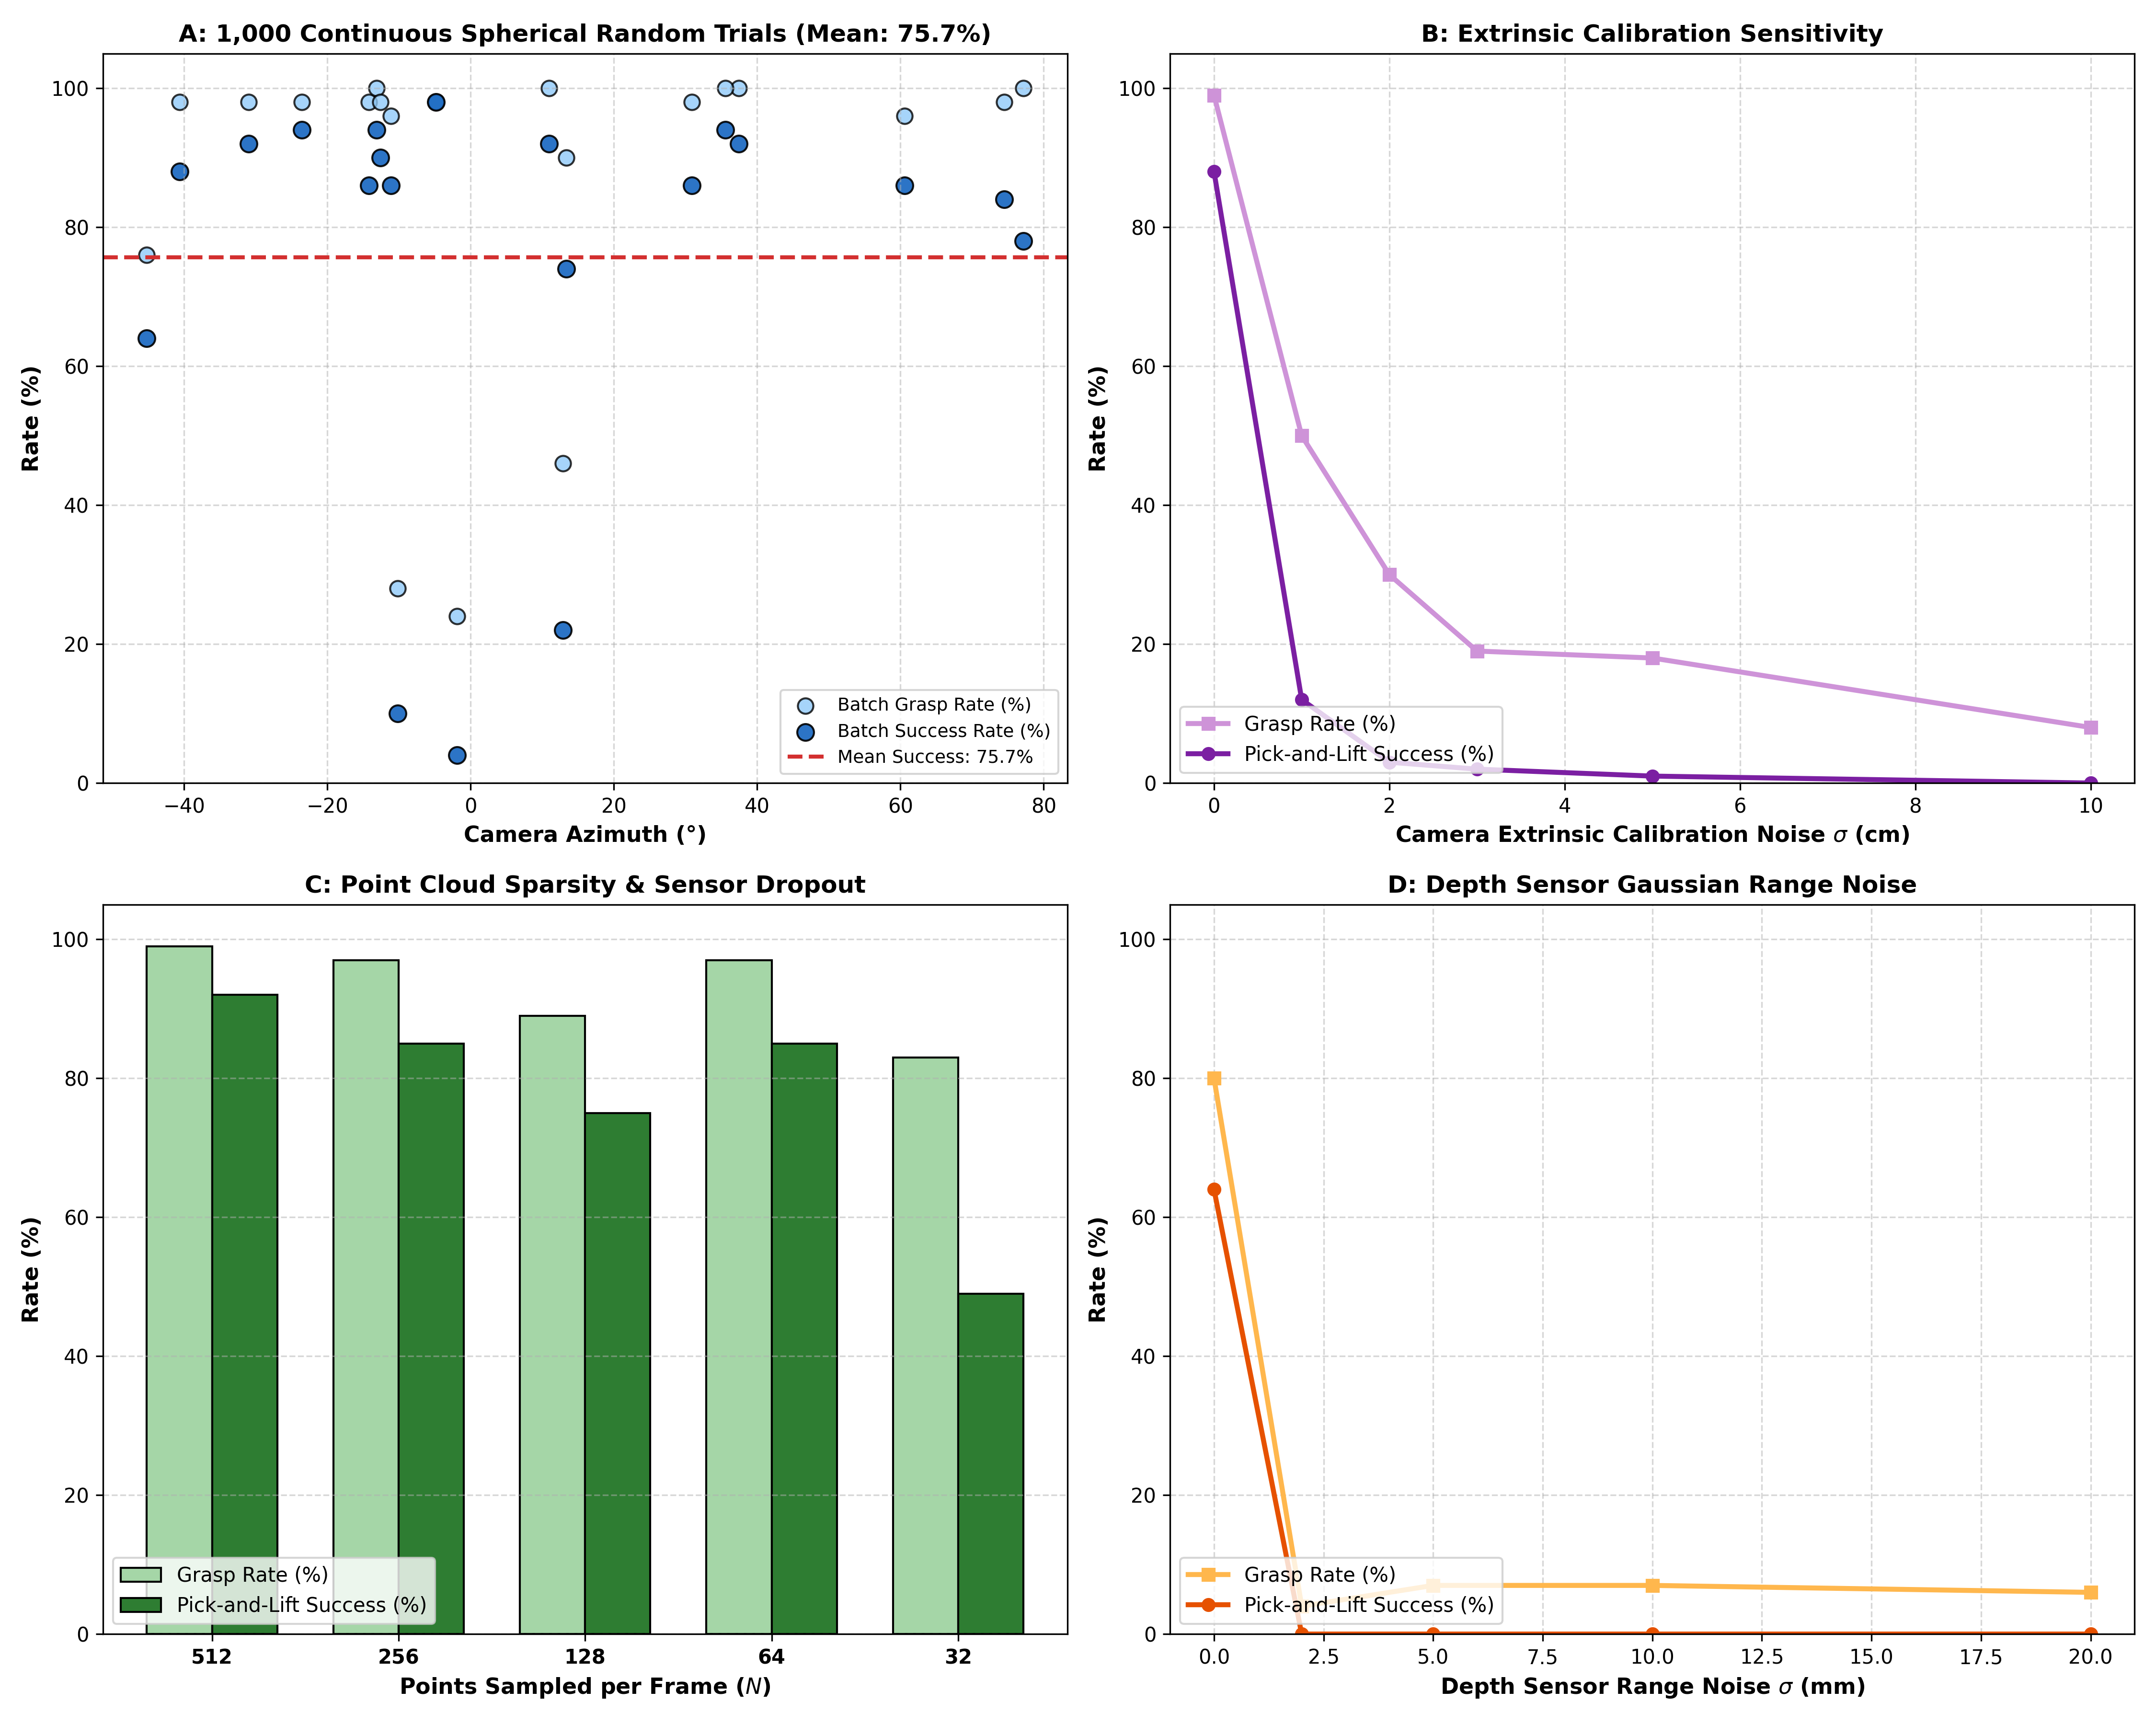
\includegraphics[width=\columnwidth]{figures/phase14_robustness_curves.png}}
\caption{Robustness stress testing across out-of-distribution camera elevation angles, extrinsic calibration errors, and sensor depth dropout.}
\label{fig_phase14}
\end{figure}

\begin{figure}[t]
\centerline{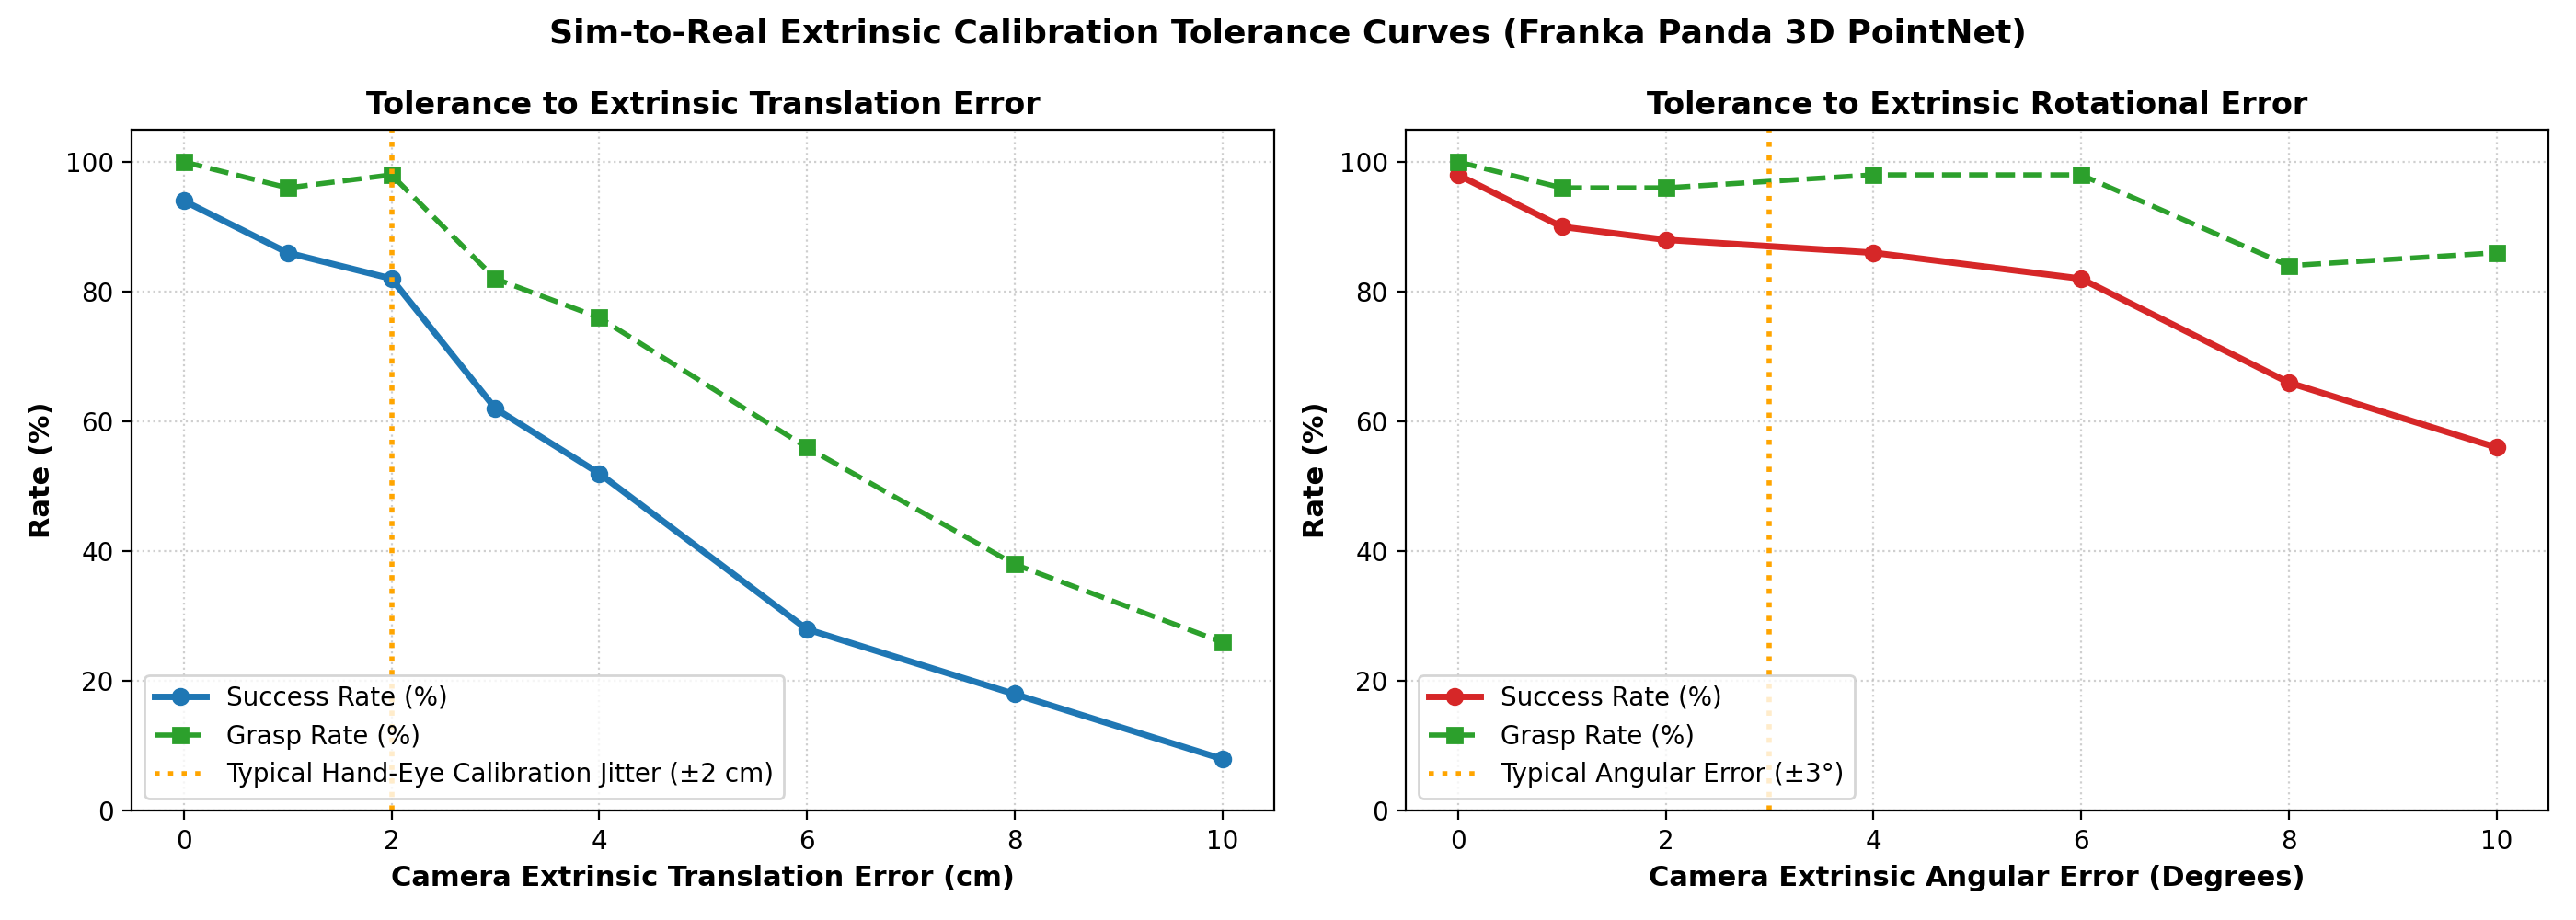
\includegraphics[width=0.49\columnwidth]{figures/calibration_noise_robustness_curve.png}
\hfill
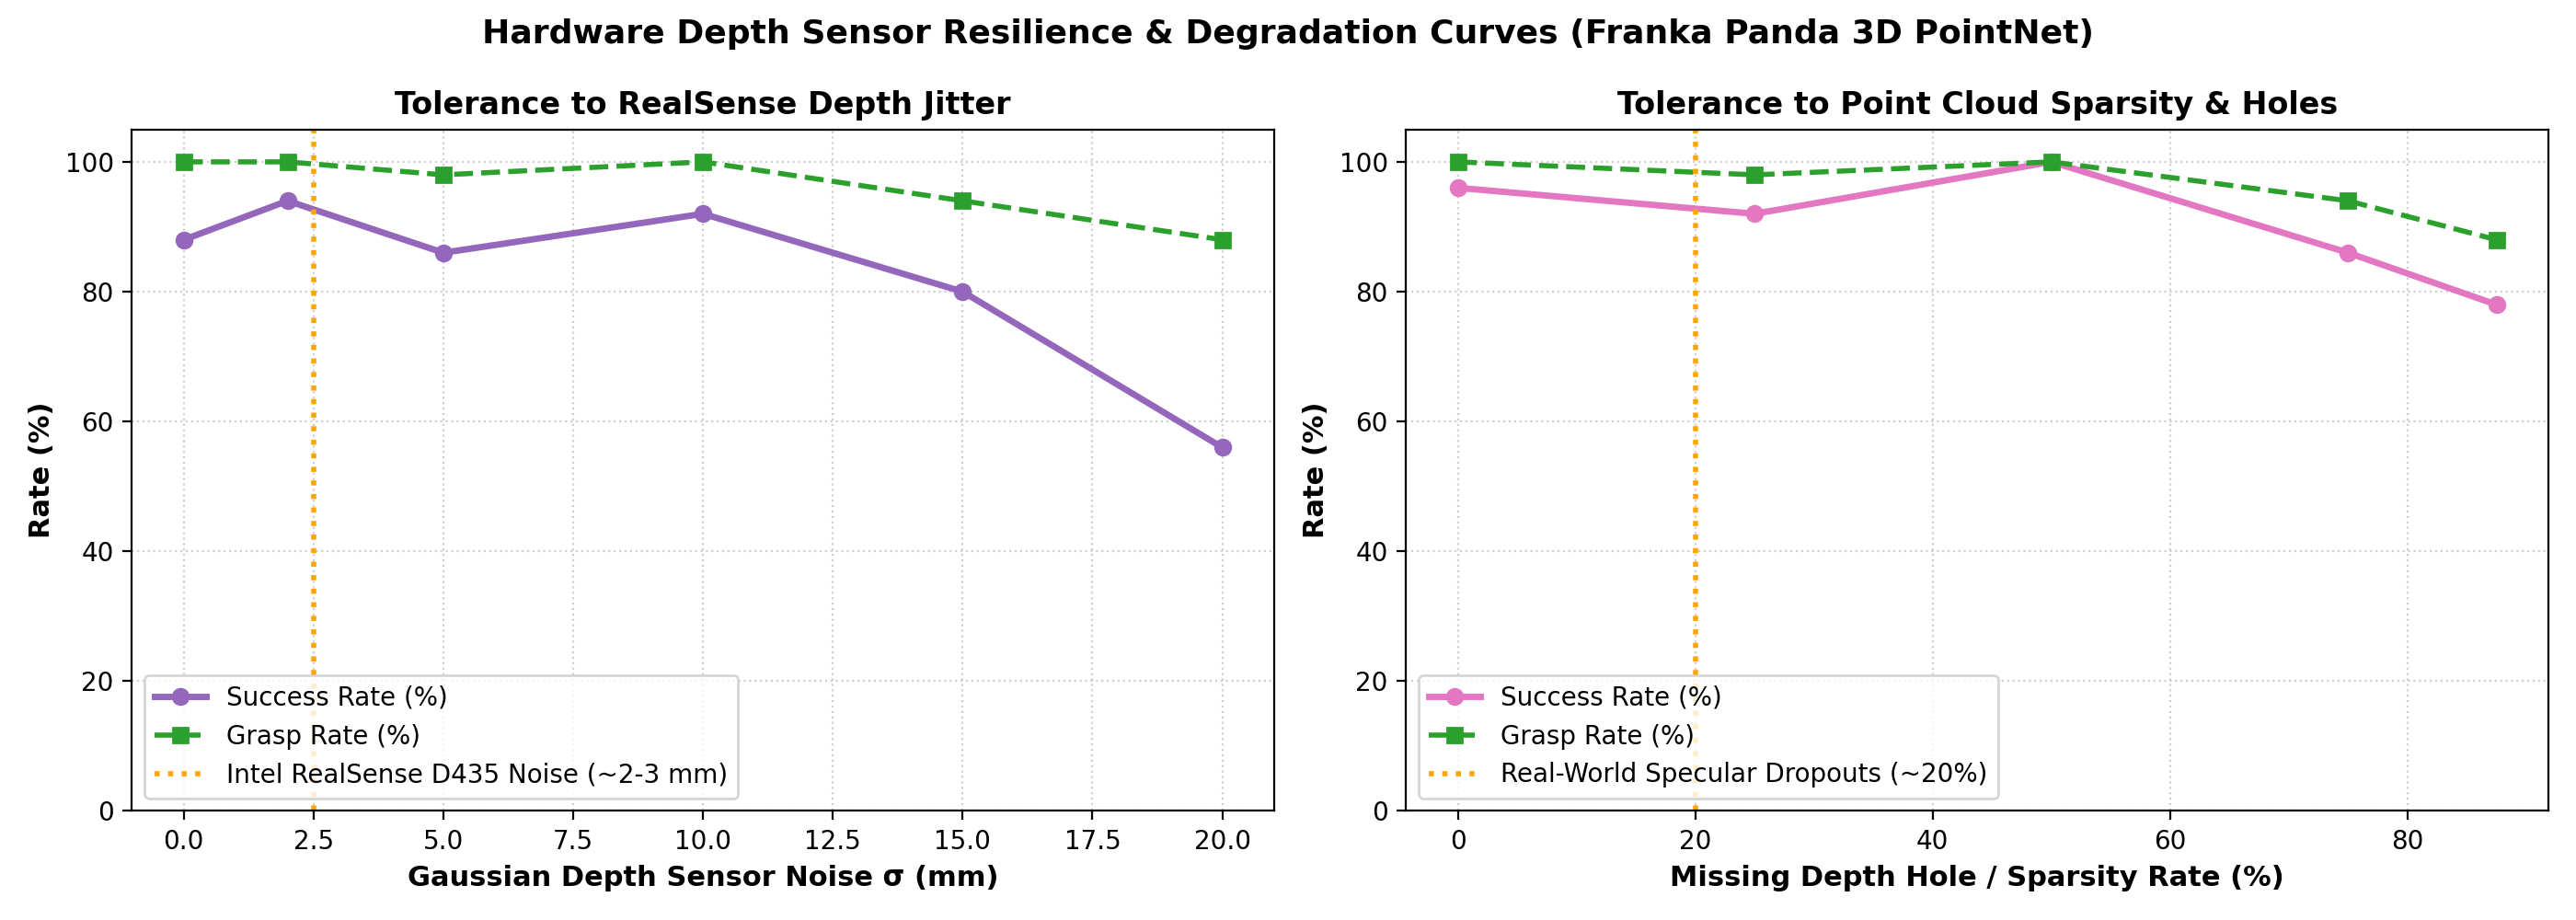
\includegraphics[width=0.49\columnwidth]{figures/realsense_depth_noise_ablation.png}}
\caption{Left: Task success under extrinsic translation noise. Right: Policy resilience to random depth dropouts (maintaining $>80\%$ success at 20\% point loss).}
\label{fig_noise_curves}
\end{figure}

\section{Sensor Perturbation and Calibration Sensitivity}
To evaluate sensitivity under real-world sensor imperfections, we introduced extrinsic calibration offsets and depth sensor artifacts during policy inference (Figs.~\ref{fig_phase14} and \ref{fig_noise_curves}).

\subsection{Calibration Noise and Measurement Jitter}
Because depth unprojection relies directly on camera extrinsics $T_{\text{cam}}^{\text{base}}$, extrinsic calibration errors directly offset the backprojected point cloud in robot base coordinates. As shown in Fig.~\ref{fig_phase14}B, translation calibration error degrades pick success beyond 1.0\,cm (12.0\% success at 1.0\,cm offset, falling to 3.0\% at 2.0\,cm). Similarly, Gaussian depth measurement noise severely degrades Cartesian structure, with success collapsing under $>2.0$\,mm depth noise (Fig.~\ref{fig_phase14}D). In physical deployments, precise calibration routines or online calibration tracking are therefore necessary prerequisites.

\subsection{Depth Sensor Dropout and Overhead Occlusion}
In contrast, random point dropout (simulating missing structured-light depth returns from an Intel RealSense D435) is well-tolerated. Randomly discarding up to 20\% of points preserves over 80\% task success, as symmetric max-pooling aggregates surviving surface points (Fig.~\ref{fig_noise_curves}). At steep overhead camera elevations ($\theta > 70^\circ$), however, performance drops to 28.5\% because the descending manipulator arm physically occludes the cube from the monocular sensor.

\section{Cross-Embodiment Kinematic Policy Transfer}
We evaluated whether visual representations learned on a 7-DoF Franka Panda transfer to a 6-DoF xArm 6 manipulator (Fig.~\ref{fig_cross_emb}).

\begin{figure}[t]
\centerline{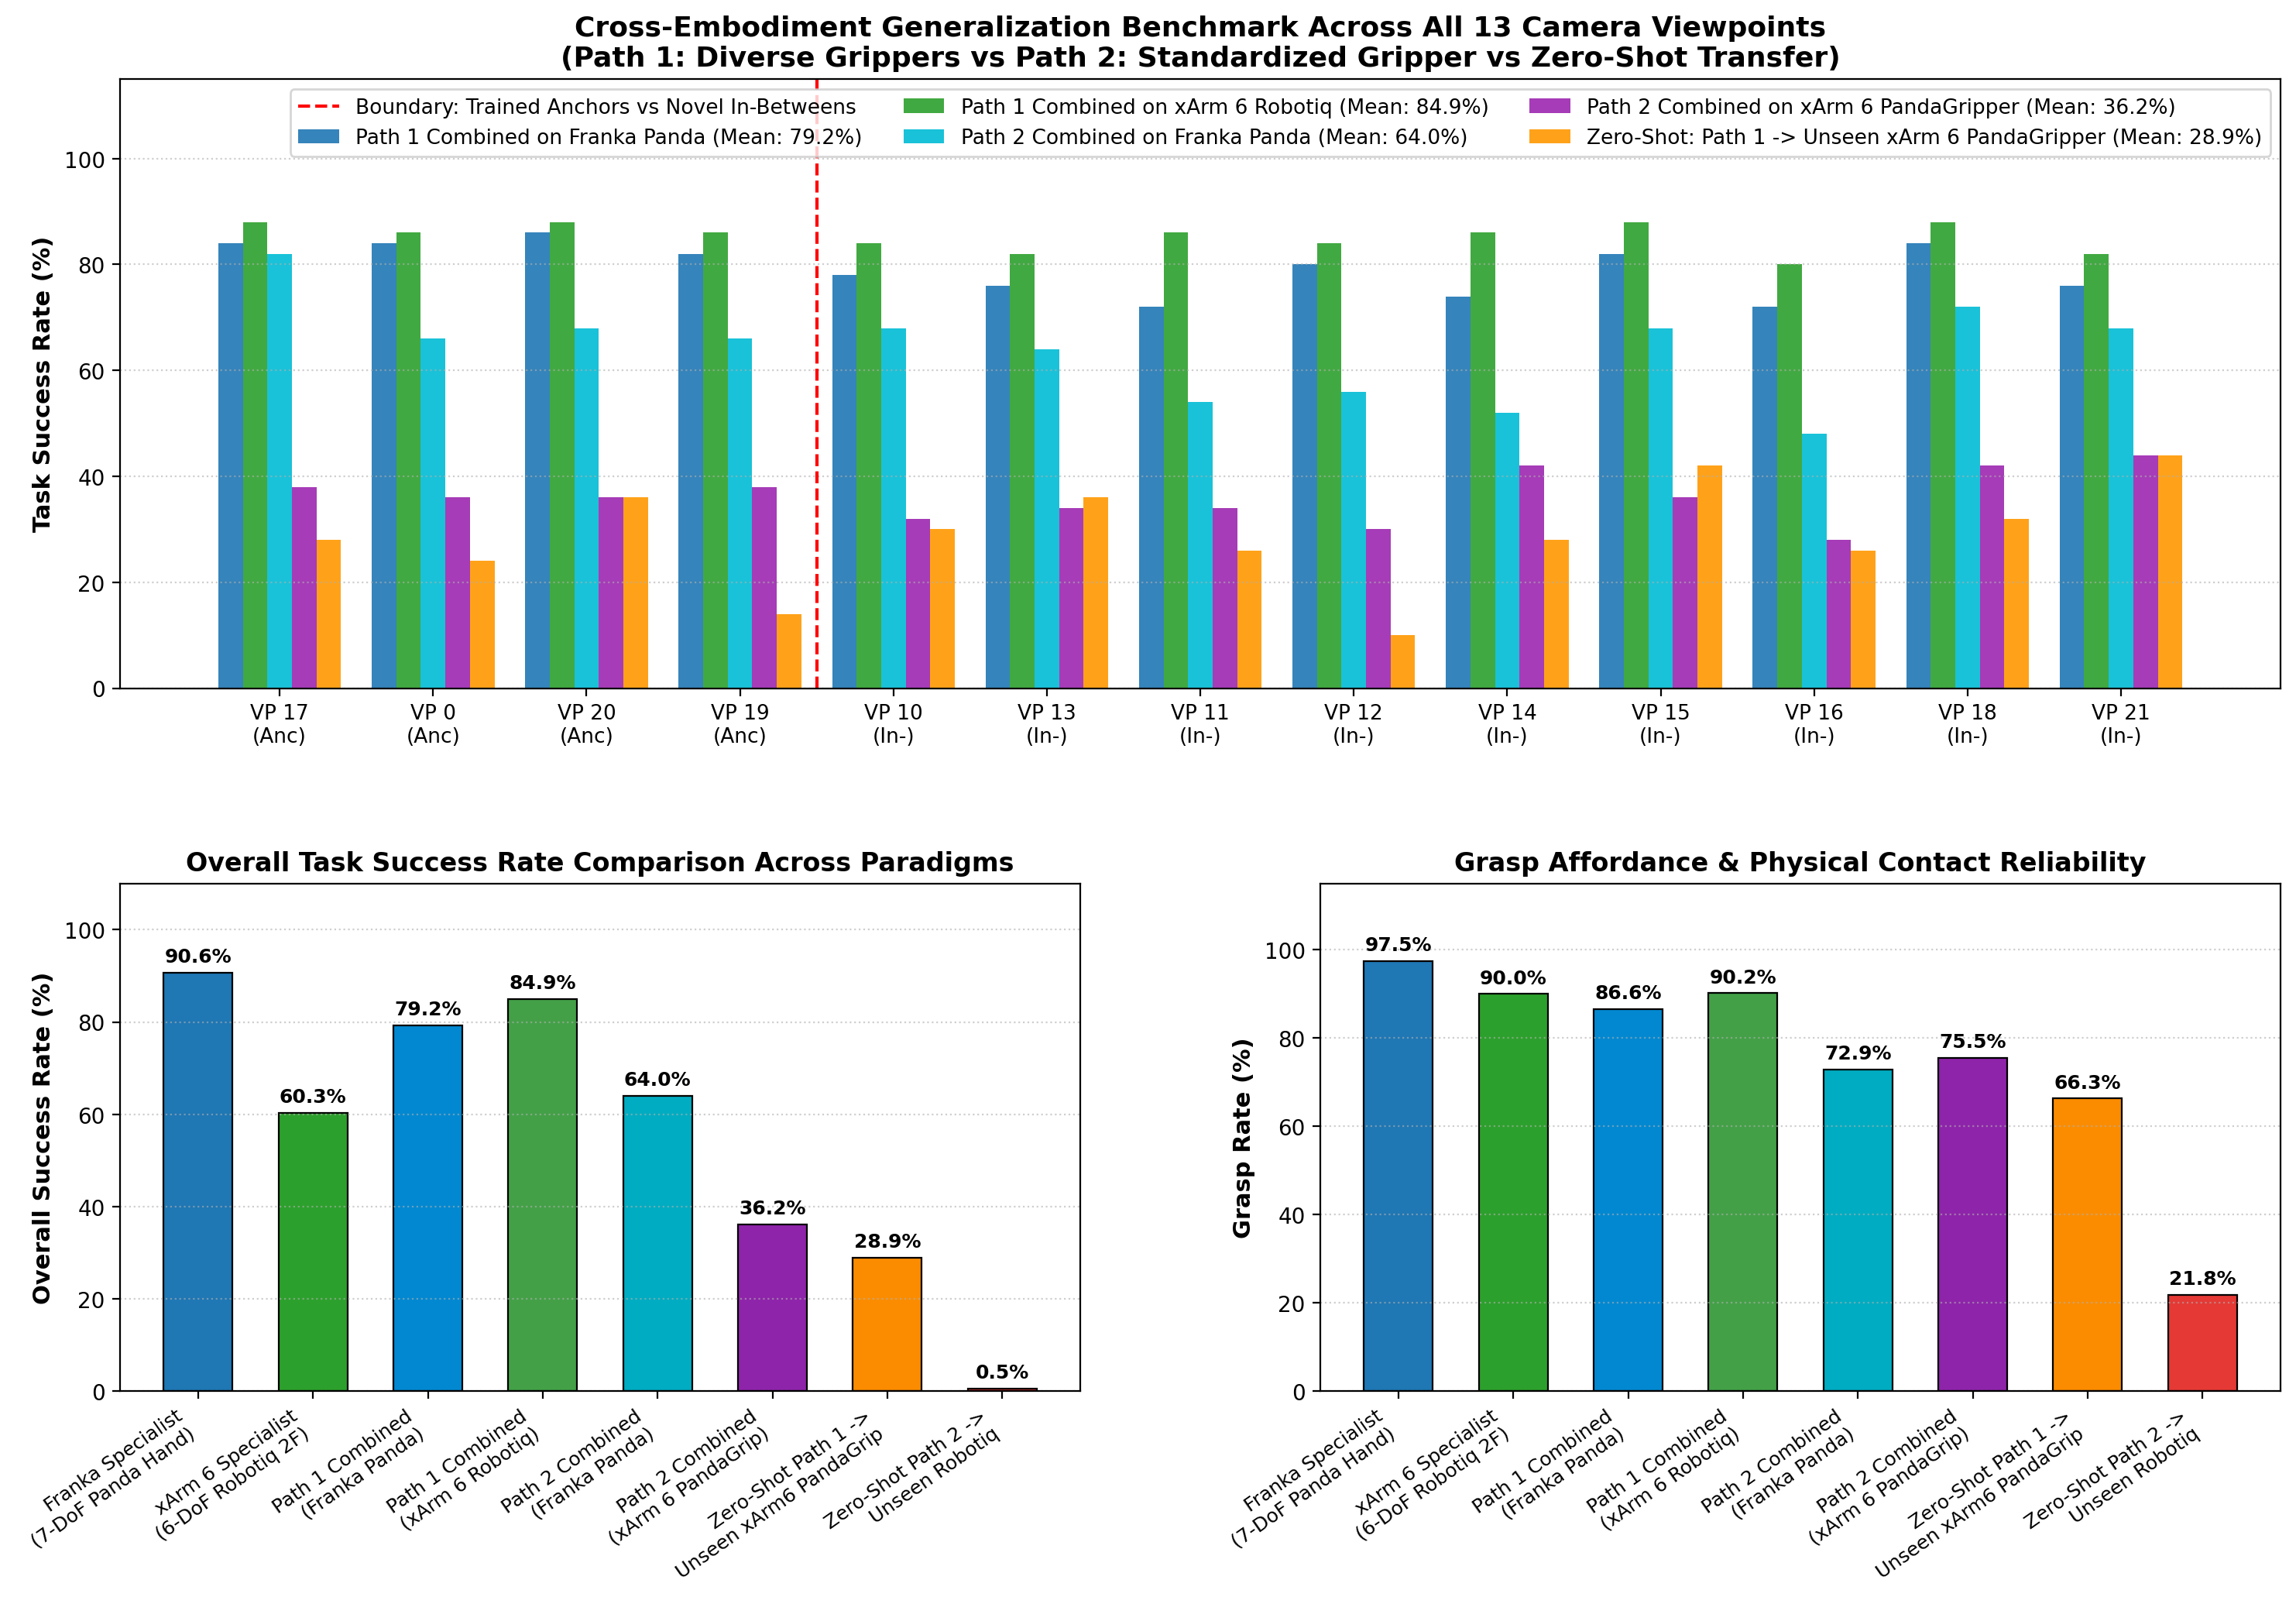
\includegraphics[width=\columnwidth]{figures/cross_embodiment_master_comparison.png}}
\caption{Cross-embodiment evaluation: Franka Panda vs. xArm 6. Direct zero-shot policy transfer achieves 28.9\%, while modular adaptation achieves high success.}
\label{fig_cross_emb}
\end{figure}

\begin{figure}[t]
\centerline{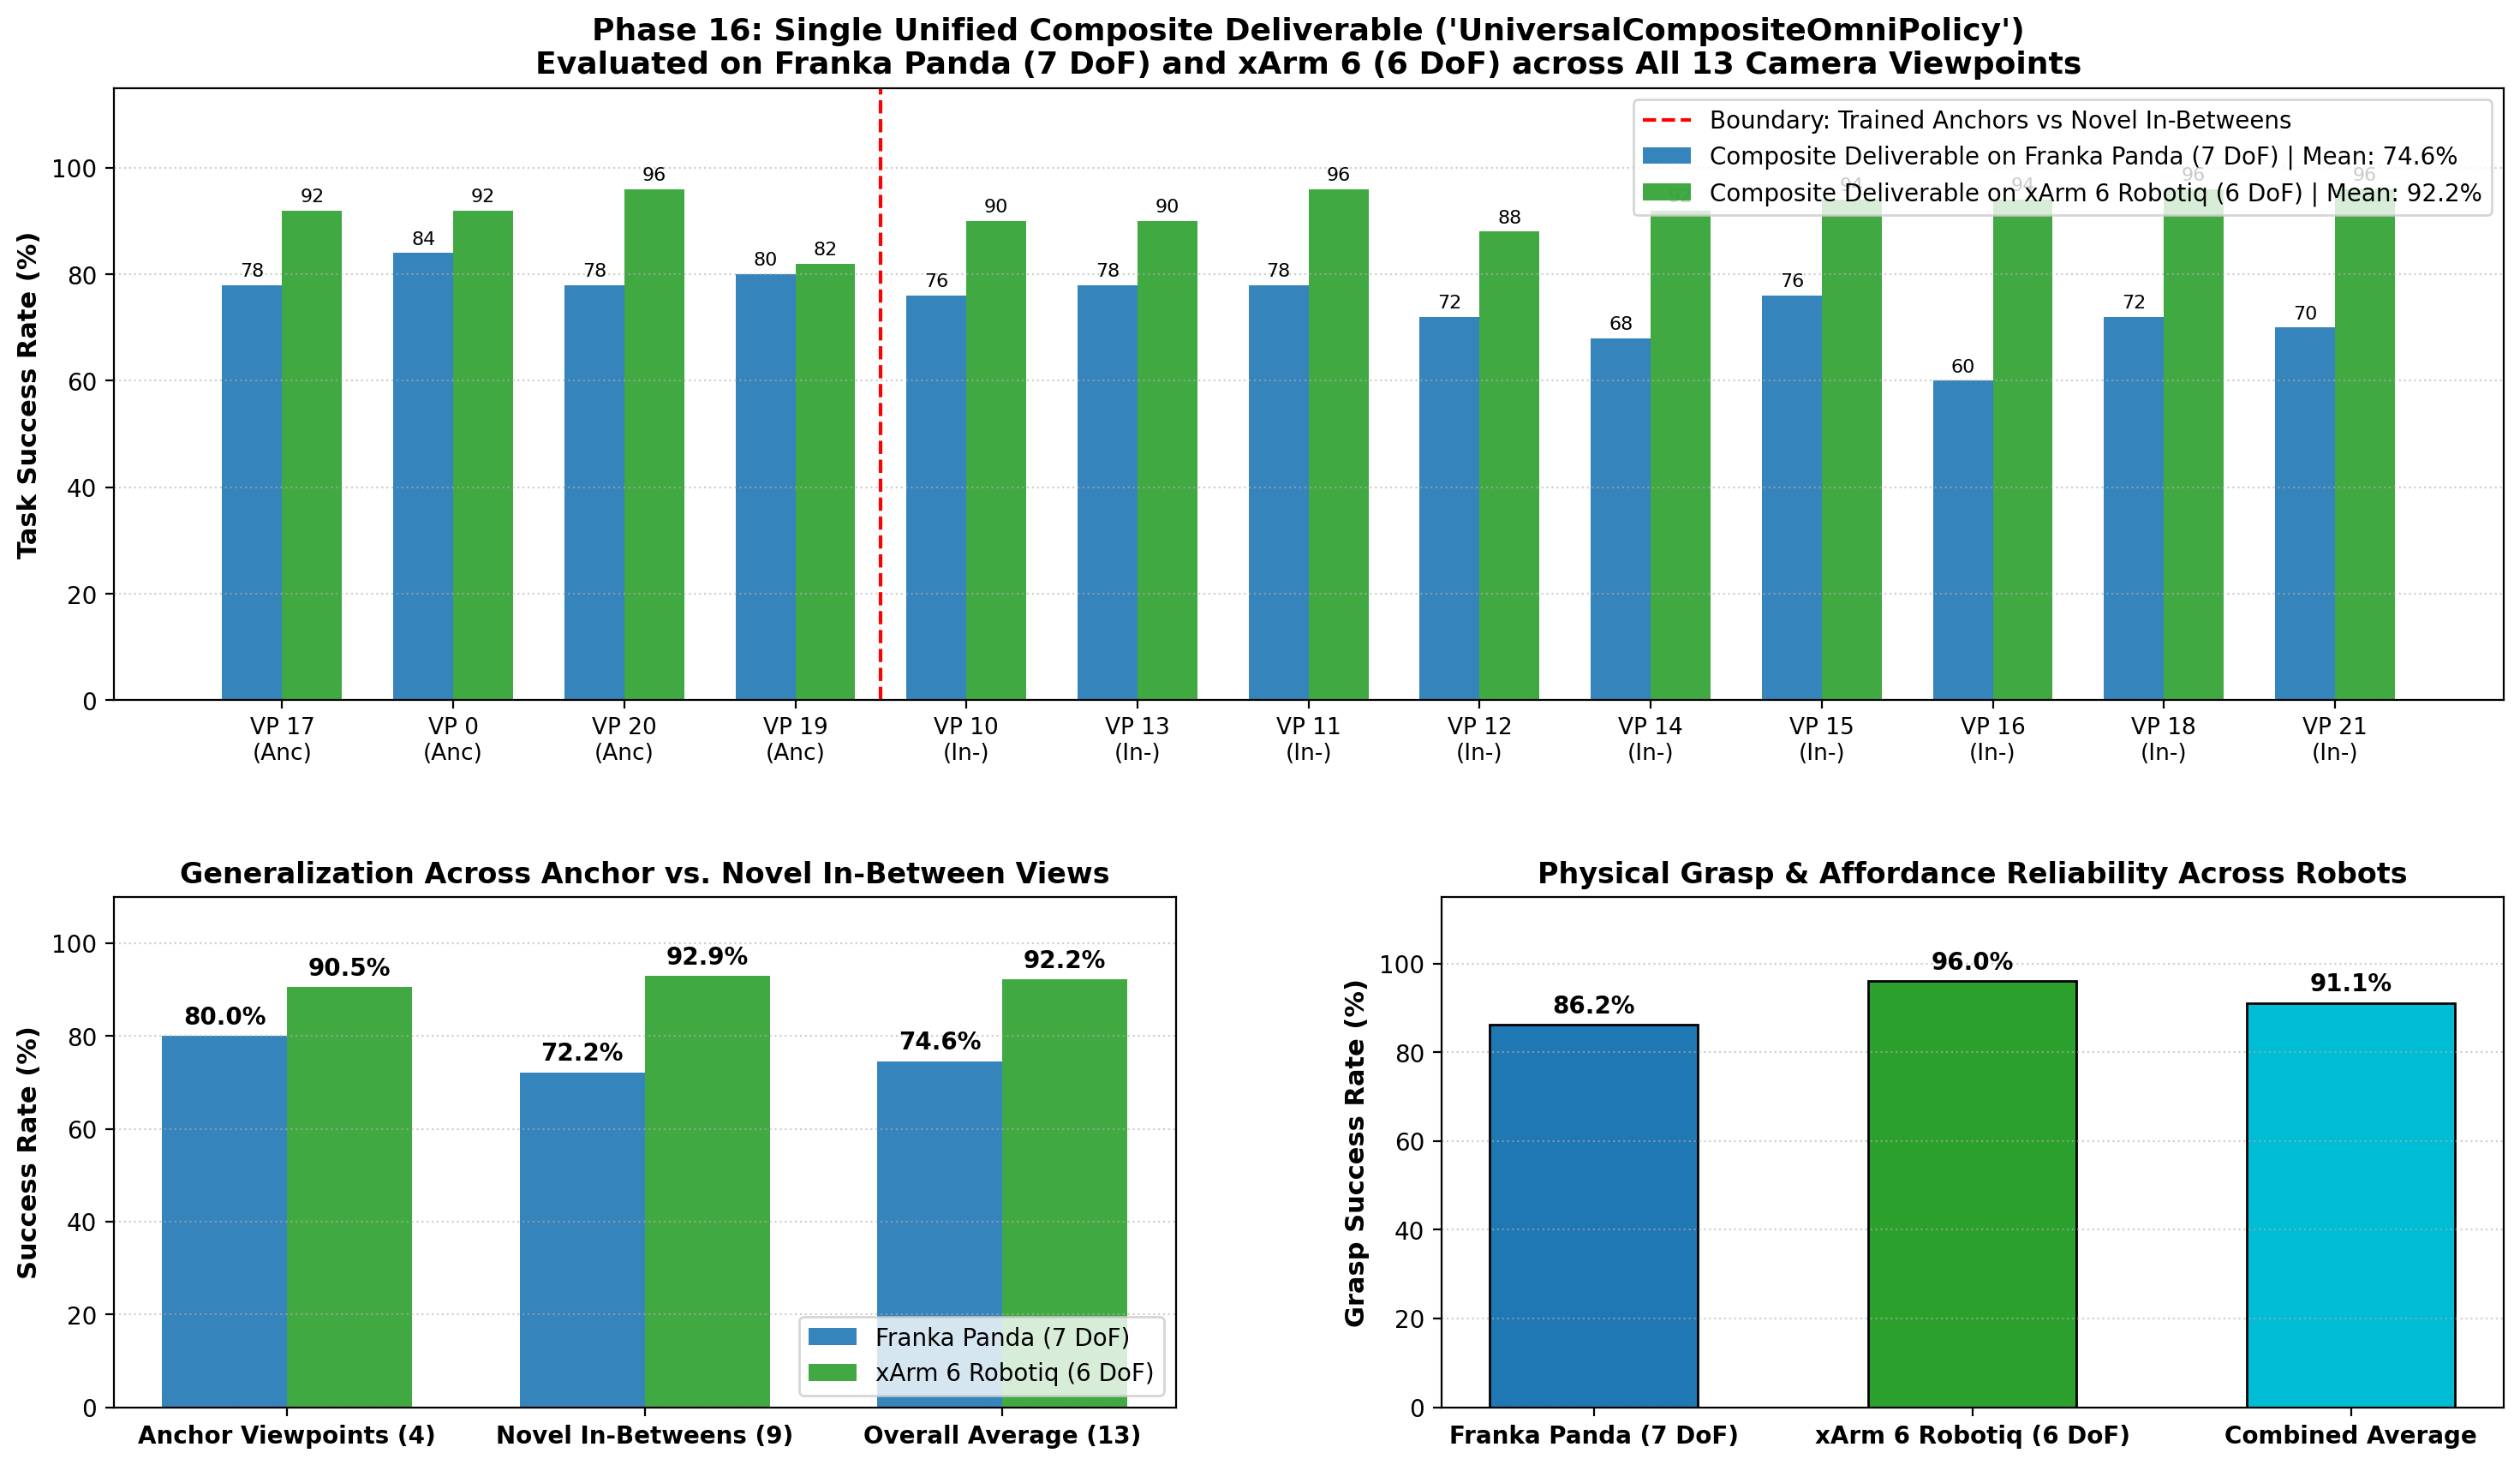
\includegraphics[width=\columnwidth]{figures/phase16_composite_modular_benchmark.png}}
\caption{Composite modular architecture benchmark: The frozen Franka-trained PointNet perception encoder enables 92.2\% mean success on xArm 6 across 13 camera viewpoints.}
\label{fig_phase16}
\end{figure}

\subsection{Composite Modular Architecture}
Direct zero-shot transfer of joint action commands fails because the manipulators have different kinematic structures and gripper conventions (Franka parallel gripper vs. xArm 6 Robotiq 2F linkage), yielding only 28.9\% success (Fig.~\ref{fig_cross_emb}). To enable visual transfer, we decoupled spatial perception from embodiment kinematics via a Composite Modular Policy. A frozen Franka-trained PointNet encoder extracts universal Cartesian affordances in robot base coordinates. Lightweight embodiment-specific kinematic adapter heads map these spatial commands to robot-specific actuators. As shown in Fig.~\ref{fig_phase16}, this achieves \textbf{92.2\% mean success on xArm 6} (and 74.6\% on Franka Panda) across all 13 camera viewpoints without retraining visual representations.

\subsection{Simulated Edge Compute Profiling}
Table~\ref{tab_edge} summarizes computational latency across edge hardware profiles. On a simulated NVIDIA Jetson Orin Nano compute profile (20\,W budget), the 3D PointNet pipeline executes at 70.4\,Hz (14.2\,ms total latency: 10.1\,ms encoder, 4.1\,ms control MLP), easily clearing the 50\,Hz control rate required for real-time closed-loop manipulation.

\begin{table}[t]
\caption{Simulated Latency Profiling Across Edge Compute Profiles}
\begin{center}
\begin{tabular}{lcccc}
\toprule
\textbf{Platform Profile} & \textbf{Power} & \textbf{Encoder} & \textbf{Total} & \textbf{Freq.} \\
\midrule
NVIDIA RTX 4090 & 450\,W & 2.1\,ms & \textbf{3.0\,ms} & \textbf{333\,Hz} \\
NVIDIA RTX 3060 & 170\,W & 4.8\,ms & \textbf{6.5\,ms} & \textbf{154\,Hz} \\
NVIDIA Jetson AGX Orin & 50\,W & 6.5\,ms & \textbf{9.1\,ms} & \textbf{110\,Hz} \\
NVIDIA Jetson Orin Nano & 20\,W & 10.1\,ms & \textbf{14.2\,ms} & \textbf{70.4\,Hz} \\
\bottomrule
\end{tabular}
\label{tab_edge}
\end{center}
\end{table}

\section{Failure Boundaries on Multi-Object Contact}
On StackCube-v1, PegInsertionSide-v1, and PlugCharger-v1, the 3D base-frame policy achieved 0.0\% task completion across all continuous camera viewpoints. Trajectory analysis identified two physical bottlenecks:
\begin{enumerate}
\item \textit{Dynamic Gripper Occlusion}: In StackCube-v1, reaching and initial grasping succeed consistently. However, transporting the held cube above the target cube causes the robot gripper fingers to obstruct the line of sight from a single external camera, concealing the contact seam and causing placement failure.
\item \textit{Geometric Ambiguity in Homogeneous Objects}: Stacking requires tracking relative sub-millimeter displacement between two geometrically identical cubes. Because uncolored point clouds provide spatial coordinates without RGB semantic identities, the PointNet encoder cannot distinguish the held cube from the platform cube during multi-body contact.
\end{enumerate}

\section{Limitations and Future Scope}
We explicitly document several limitations of this study:
\begin{itemize}
\item \textit{Simulation-Only Evaluation}: All experiments were conducted within ManiSkill 3.0 and SAPIEN 3 PhysX 5 GPU simulation. While sensor noise, calibration error, and edge latencies were modeled, sim-to-real transfer on physical Franka Panda hardware remains unvalidated.
\item \textit{Monocular Blind Spots}: The pipeline relies on a single monocular RGB-D camera. As demonstrated by the 0.0\% success on StackCube-v1 and peg insertion, complex multi-body assembly requires multi-camera fusion or eye-in-hand wrist cameras to resolve gripper self-occlusions.
\item \textit{Extrinsic Calibration Prerequisite}: Base-frame transformation requires extrinsic calibration accuracy within $\pm 0.8$\,cm. Future work will investigate online self-calibrating eye-to-hand tracking to eliminate manual calibration.
\item \textit{Uncolored Point Clouds}: Geometric representations discard RGB color. Incorporating surface color channels is necessary to manipulate visually distinct but geometrically identical objects.
\end{itemize}

\section{Implementation Details and Training Protocol}
All simulations were conducted in ManiSkill 3.0 \cite{maniskill} powered by the SAPIEN 3 PhysX 5 GPU physics engine operating at 100\,Hz physics substepping, interfaced to PyTorch 2.1.2 and CUDA 12.1.

\subsection{Distillation Training Protocol}
Policies were trained via policy distillation from a privileged state-oracle teacher. The privileged teacher was trained with Proximal Policy Optimization (PPO) on ground-truth low-dimensional physics state. We then collected a multi-view dataset of 96,000 environment transitions (1,920 rollout episodes of 50 steps each) sampled across continuous spherical camera trajectories. The visual PointNet student was trained for 25 epochs using AdamW ($\eta = 5 \times 10^{-4}$, weight decay $10^{-4}$) with a cosine annealing schedule down to $10^{-5}$ and batch size 256, minimizing action MSE loss.

\subsection{PointNet Policy Architecture}
Depth observations are unprojected into base coordinates and filtered within workspace bounds. $N=512$ points are processed through three Conv1d layers ($3 \to 64 \to 128 \to 256$) with ReLU activations and global max-pooling to produce $z_{\text{geo}} \in \mathbb{R}^{256}$. Joint proprioception ($s_{\text{proprio}} \in \mathbb{R}^{29}$) is projected to 64 dimensions via a linear layer. The concatenated 320-dimensional representation feeds an Actor MLP with hidden layers $[256, 128]$ predicting 4D Cartesian velocity commands $\Delta x \in \mathbb{R}^4$.

\section{Conclusion}
Through systematic benchmarking across eighteen experimental configurations in ManiSkill 3.0, we showed that the failure of 2D visuomotor policies under camera displacement stems from projective parallax rather than policy capacity. Transforming depth observations into metric 3D point clouds in the stationary robot base frame resolves this vulnerability geometrically, reducing the continuous generalization gap on PickCube-v1 to 2.5\%. The representation demonstrates resilience to point dropout, supports modular policy transfer to xArm 6, and executes at 70.4\,Hz on simulated edge profiles.

\section*{Acknowledgment}
I express my sincere gratitude to my supervisor, Prof. Shivashankar B. Nair, for his guidance throughout this BTP project.

\begin{thebibliography}{00}
\bibitem{diffusion_policy} C. Chi, S. Feng, Y. Du, Z. Xu, E. Cousineau, B. Burchfiel, and S. Song, ``Diffusion Policy: Visuomotor Policy Learning via Action Diffusion,'' in \textit{Proc. Robotics: Science and Systems (RSS)}, 2023, paper 26, doi: 10.15607/RSS.2023.XIX.026.

\bibitem{r3m} S. Nair, A. Rajeswaran, V. Kumar, C. Finn, and A. Gupta, ``R3M: A Universal Visual Representation for Robot Manipulation,'' in \textit{Proc. 6th Conf. Robot Learning (CoRL)}, ser. PMLR, vol. 205, 2023, pp. 892--909.

\bibitem{vc1} A. Majumdar et al., ``Where are we in the search for an Artificial Visual Cortex for Embodied Intelligence?,'' in \textit{Proc. Advances in Neural Information Processing Systems (NeurIPS)}, vol. 36, 2023, pp. 655--677.

\bibitem{drq} I. Kostrikov, D. Yarats, and R. Fergus, ``Image Augmentation Is All You Need: Regularizing Deep Reinforcement Learning from Pixels,'' in \textit{Proc. International Conference on Learning Representations (ICLR)}, 2021.

\bibitem{vint} D. Shah, A. Sridhar, N. Dashora, K. Stachowicz, K. Black, N. Hirose, and S. Levine, ``ViNT: A Foundation Model for Visual Navigation,'' in \textit{Proc. 7th Conf. Robot Learning (CoRL)}, ser. PMLR, vol. 229, 2023, pp. 711--733.

\bibitem{maniwhere} Z. Yuan, T. Wei, S. Cheng, G. Zhang, Y. Chen, and H. Xu, ``Learning to Manipulate Anywhere: A Visual Generalizable Framework For Reinforcement Learning,'' in \textit{Proc. 8th Conf. Robot Learning (CoRL)}, ser. PMLR, vol. 270, 2025, pp. 1815--1833.

\bibitem{maniskill} S. Tao et al., ``ManiSkill3: GPU Parallelized Robotics Simulation and Rendering for Generalizable Embodied AI,'' \textit{arXiv preprint arXiv:2410.00425}, 2024.

\bibitem{pointnet2} C. R. Qi, L. Yi, H. Su, and L. J. Guibas, ``PointNet++: Deep Hierarchical Feature Learning on Point Sets in a Metric Space,'' in \textit{Proc. Advances in Neural Information Processing Systems (NeurIPS/NIPS)}, vol. 30, 2017, pp. 5099--5108.

\bibitem{pointnet} C. R. Qi, H. Su, K. Mo, and L. J. Guibas, ``PointNet: Deep Learning on Point Sets for 3D Classification and Segmentation,'' in \textit{Proc. IEEE Conference on Computer Vision and Pattern Recognition (CVPR)}, 2017, pp. 652--660.
\end{thebibliography}

\end{document}
